%% v3.0 [2015/11/14]
%\documentclass[Proof,technicalreport]{ieicej}
\documentclass[technicalreport]{ieicej}
%\usepackage{graphicx}
\usepackage[T1]{fontenc}
\usepackage{lmodern}
\usepackage{textcomp}
\usepackage{latexsym}
%\usepackage[fleqn]{amsmath}
%\usepackage{amssymb}

\usepackage[dvipdfmx]{graphicx,xcolor}
\usepackage{colortbl}
\usepackage{comment}
\usepackage{hhline}
\usepackage{url}


\def\IEICEJcls{\texttt{ieicej.cls}}
\def\IEICEJver{3.0}
\newcommand{\AmSLaTeX}{%
 $\mathcal A$\lower.4ex\hbox{$\!\mathcal M\!$}$\mathcal S$-\LaTeX}
%\newcommand{\PS}{{\scshape Post\-Script}}
\def\BibTeX{{\rmfamily B\kern-.05em{\scshape i\kern-.025em b}\kern-.08em
 T\kern-.1667em\lower.7ex\hbox{E}\kern-.125em X}}

\jtitle{開発標準プロセスを用いた不完全なソフトウェア要求に対する問題検出の分類法}
%\jsubtitle{技術研究報告原稿のための解説とテンプレート}
\etitle{Classification of problem detection for incomplete software requirements using the development standard process}
\authorlist{%
 \authorentry[miyamura.toma.mo6@is.naist.jp]{宮村 純真}{Toma Miyamura}{NAIST}
 \authorentry[]{川口 真司}{Shinji Kawaguchi}{JAXA}
 \authorentry[]{石濱 直樹}{Naoki Ishihama}{JAXA}
 \authorentry[]{柿本 和希}{Kazuki Kakimoto}{JAXA}
 \authorentry[]{飯田 元}{Hajimu Iida}{NAIST}
 \authorentry[]{片平 真史}{Masafumi Katahira}{JAXA}
}
\affiliate[NAIST]{奈良先端科学技術大学院大学 情報科学研究科\hskip1zw
  〒630--0192 奈良県生駒市高山町8916--5}
 {Nara Institute of Science and Technology
Takayama-cho 8916-5, Ikoma-shi, Nara, 630-0192 Japan}

\affiliate[JAXA]{宇宙航空研究開発機構\hskip1zw
〒305--8505茨城県つくば市千現2--1--1}
 {Japan Aerospace eXploration Agency\hskip1em
Sengen 2--1--1 Tukuba-shi,
 305--8505 JAPAN}

%\MailAddress{$\dagger$hanako@denshi.ac.jp,
% $\dagger\dagger$\{taro,jiro\}@jouhou.co.jp}

\begin{document}
\begin{jabstract}
�F���@�̃\�t�g�E�F�A�ɂ����āA�\�t�g�E�F�A�̕s��̓~�b�V�����̐����ɑ΂��đ傫�ȖW���ƂȂ��Ă���B
�{�����ł̓\�t�g�E�F�A�s��̑傫�Ȍ����ƂȂ��Ă���v���R��ɒ��ڂ����B
���ۂɉF���@�Ŕ��������\�t�g�E�F�A�̕s������ɁA���ׂ̕��ނƊJ���W���v���Z�X�̂Q�‚̊ϓ_����s��̕��ނ��s���Ă���B
���̕��ނ��s�����ƂŁA�ǂ̂悤�ȕs��������̂��A�ǂ̃v���Z�X�ɂ����ĕs����������₷���̂������m�ɂȂ�B


\end{jabstract}
\begin{jkeyword}
アスキー版p\LaTeXe{},タイピングの注意事項
\end{jkeyword}
\begin{eabstract}
Software faults in spacecraft software can largely obstruct the chance of missions success.
In this research, we focus on the omitted requirement which is considered to be a major cause of software faults.
From the two perspectives of fault classification and standard development process, we classified software faults that we retrieved from actual spacecraft project(artificial satellite and rockets).
By carrying out this classification, it becomes clear which kind of process leads to more faults.

\end{eabstract}
\begin{ekeyword}
p\LaTeXe\ class file, typesetting
\end{ekeyword}
\maketitle

\section{はじめに}
�V�X�e���J���̍ۂɁC�\�t�g�E�F�A�������Ŕ�������s��͑傫��2�p�^�[���ɕ����邱�Ƃ��ł���D
1�–ڂ�``���߂��Ă���v���͐��������C�\�t�g�E�F�A�̎���������Ă���''�p�^�[���ł���C2�–ڂ�``�����͗v���ʂ�ł��邪�C�v�����s���S�ł���''�p�^�[���ł���D
�O�҂̃\�t�g�E�F�A�̎����ɂ�������̓c�[���Ȃǂ�p���邱�ƂŔ����ł���D
����ŁC��҂Ɋւ��ẮC�c�[�������݂����C�v���d�l�����ɂ��L�ڂ���Ă��Ȃ����ߔ���������ł���D
�܂��C�\�t�g�E�F�A�̎����ɂ�����s��̊����͔��ɏ��Ȃ����Ƃ����������Ŗ��炩�ɂ��Ă���\cite{4812749}�D
����āC�\�t�g�E�F�A�̐M���������߂邽�߂ɂ́C�\�t�g�E�F�A�̎����ɂ��s������łȂ��C�v���R��ɂ��s��ɂ����Ă��l������K�v������D

Avizienis��́C�s��S�̗̂v����1�‚ł��錇�ׂɊւ��镪�ޖ@���Ă��Ă���\cite{1335465}�D
�������C�ÓI�Ȍ��ׂ̕��ނ����ł́C�ڍׂȌ�����Nj����邱�Ƃ��ł����C�v�����s���S�ł��鎖�ۂɑ΂��Ă͔���������ł���D
����Ė{�����ł́C���I�ł���J���H���i�v���Z�X�j�ɒ��ڂ��邱�ƂŁC�v�����s���S�ł��邱�Ƃɑ΂��āC�Ώ��􂪔����ł���ƍl�����D

�{�����ł́C�F���@�ƌĂ΂��C�l�H�q���⃍�P�b�g�ȂǂŎ��ۂɔ���������������ƂɁC���ׂ̕��ނƊJ���H���ł���v���Z�X��2�‚̊ϓ_����s��̕��ށE���͂��s�����D
���̕��͂ɂ��C�ΏۃV�X�e���ɂ����āC�ǂ̂悤�Ȍ��ׂɊ�Â��s��������̂��C�܂��قȂ�v���Z�X�ɂɂ����ĉe�����y�ڂ��Ă���̂͂ǂ�ł��邩�����m�ɂȂ�ƍl������D

�{�_���̍\�����ȉ��Ɏ����D
2�͂ł͌����̔w�i�ɂ‚��Đ������C3�͂Œ�Ă��镪�ނ̘g�g�݂ɂ‚��ďq�ׂ�D
4�͂ł͎��ۂɃf�[�^��K�p�������ʂ��q�ׁC5�͂ōl�@�C6�͂ł܂Ƃ߂⍡��̉ۑ�ɂ‚��ďq�ׂ�D


\section{背景}
�F���@�ƌĂ΂��A�l�H�q���⃍�P�b�g�Ȃǂ͈�x��΂��Ă��܂��Ɨe�ՂɏC�����ł��Ȃ��A���i���P���A�J�����Ԃ������A���‹��Ńe�X�g�ł��Ȃ��Ȃǂ̓���������\cite{JAXA2}\cite{JAXA3}�B
����āA�F���@�̃\�t�g�E�F�A�J���ɂ����āA�����Ɏ��s���Ȃ����̂ł��邩�A���Ȃ킿���M���������߂���͕̂K�v�s�Œ��ł��B
���M�����V�X�e���ł͏�Q�Ƃ��Č��������Ȃ��悤�ȑ΍􂪕K�v�ƂȂ�B
������������邽�߂ɁA�����̐ÓI�ȕ��ނ��s�Ă��錤�������ł͕s�\���ł���B

���̖����������邽�߂ɖ{�����ł́A���ׂɂ�镪�ޖ@�����łȂ��A���I�ȊJ���v���Z�X��p���āA�v�����s���S�ł��邱�ƂɋN������\�t�g�E�F�A���̕��ޖ@��񎦂���B
���ׂɂ�镪�ޖ@�Ƃ���Basic concepts and taxonomy of dependable and secure computing\cite{1335465}��p�����B
�v���Z�X�Ƃ��ĉF���q�󌤋��J���@�\�iJAXA�j�Ŏg�p����Ă���\�t�g�E�F�A�J���W����p�����B\cite{JAXA}




\section{提案する分類の枠組み}
�{�����łQ�‚̎w�W��p����B
�P�–ڂ́A�s��̌����ƂȂ��Ă��錇�ׂɂ‚��Ă̕��ނł���B
�Q�–ڂ́A�J���̍H���������Ă���J���v���Z�X�ł���B
���̈قȂ鎲�̂Q�‚̎w�W��g�ݍ��킹�邱�ƂŁA�����Ă��Ȃ������s��̌X���̔����‚‚Ȃ��邱�Ƃ����҂ł���B
���̏͂ł́A���ꂼ��̎w�W�ɂ‚��Đ���������B

\subsection{���ׂ̕���}
�܂����߂ɁA�s��Ƃ́A���ׂƂ͉����ɂ‚��Đ���������\cite{1335465}�B
�}\ref{�s��̊֌W}�Ɏ����悤�ɕs��Ƃ́A�{���񋟂����ׂ��A�������T�[�r�X�����炩�̉e���Ő������񋟂���Ȃ����ł���B
���̐������Ȃ��T�[�r�X��Ԃ̂��Ƃ�Failure�i��Q�j�Ƃ����B
��Q�ɂ‚Ȃ��肤��V�X�e���̓�����Ԃ�Error�i���j�Ƃ����B
��肪�����邫��������A�����ƂȂ���̂�Fault�i���ׁj�ł���B
����͂��̌��ׂɂ‚��Ē��ڂ����B

\begin{figure}
\begin{center}
\includegraphics[keepaspectratio, scale=0.2]{relationship.eps}
\caption{�s��Ɋւ��錇�ׁA���A��Q�̊֌W}
\label{�s��̊֌W}
\end{center}
\end{figure}

��s����\cite{1335465}�ł́A��ʓI�ȕs��ɂ‚��Đ�������Ă���B
���ɁA�s��S�̂̌��̌����ƂȂ錇�ׂɂ‚��Ē��ڂ��Ă���B
�}\ref{���ׂ̕���}�Q�l�̒l�����‚W�‚̊ϓ_��p���āA���v�Q�T�U�ʂ肩�猾�t�̒�`�㑶�݂��Ȃ����̂��������A�R�P�ʂ�Ō��ׂ�ԗ��I�ɕ��ނ��Ă���B
����ŁA�����ƂȂ錇�ׂ����ނł����Ƃ��Ă��A���M�����V�X�e���ɒv���I�ȉe����^����h�v���̕s���S���h�ɑΏ����邱�Ƃ͍���ł���B

\begin{figure}
\begin{center}
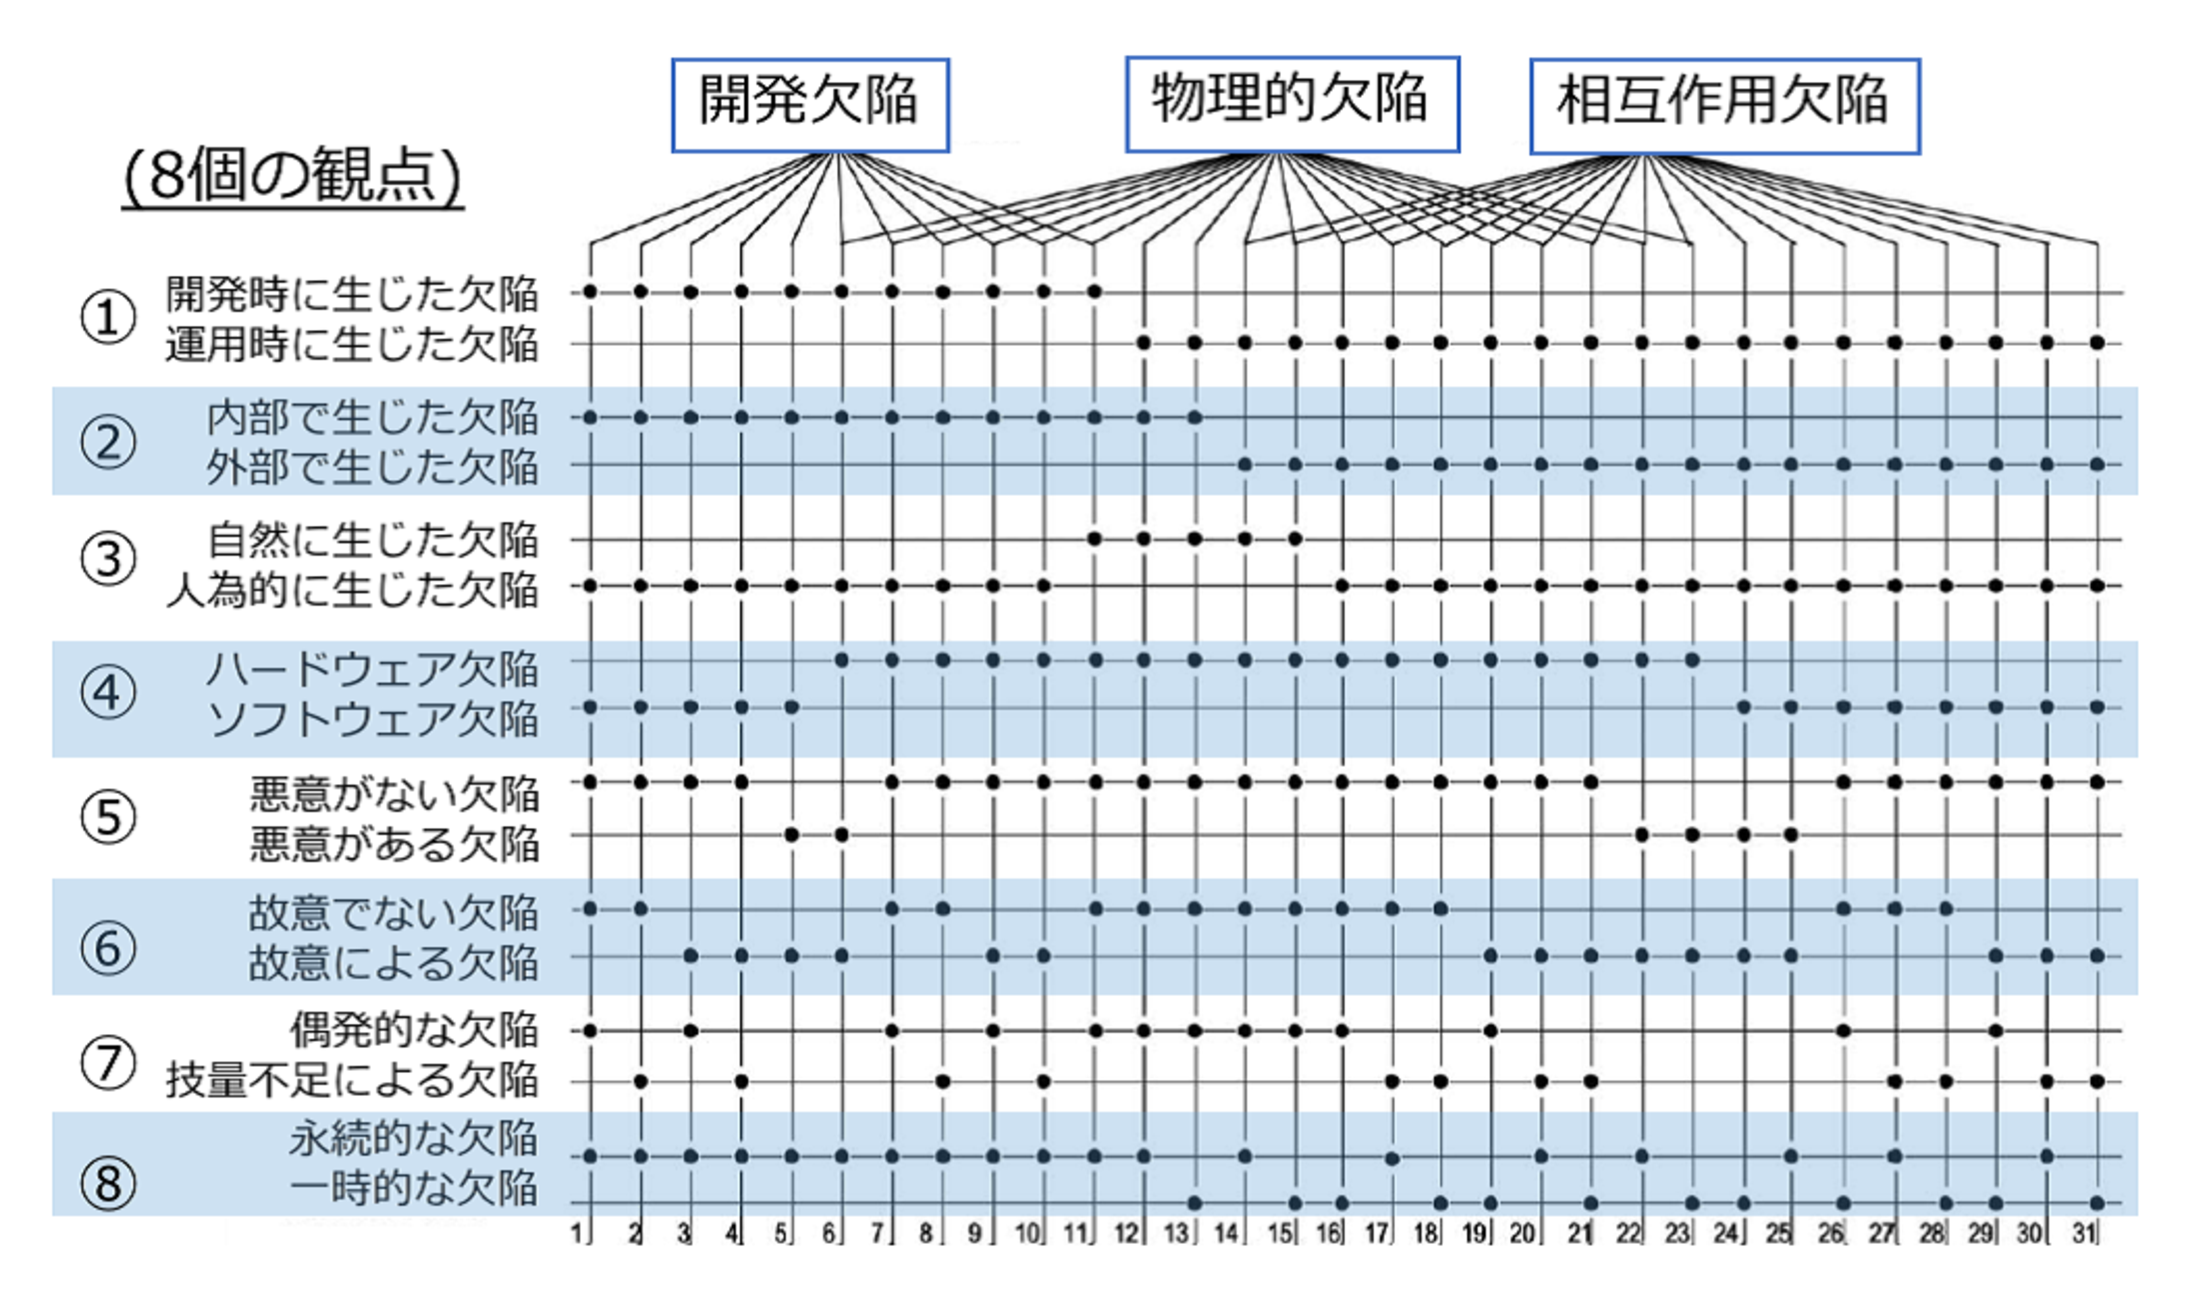
\includegraphics[keepaspectratio, scale=0.2]{classfication.eps}
\caption{���ׂ̕��ތ��ʁi�v�C���j}
\label{���ׂ̕���}
\end{center}
\end{figure}

�{�����ł́A���̕��ނ���\�t�g�E�F�A�Ɋ֌W���A����ɊJ�����ɐ��������̂ɒ��ڂ����B
���̌��ʂR�P�ʂ�̕��ނ��A�}\ref{���ׂ̕���}�Ɏ����P�`�T�Ԃ܂ł̂T�ʂ�ƂȂ����B
����ɁA�h���ӂ����錇�ׁh�͑��݂��Ȃ����̂Ƃ����B
����đΏۂƂ���̂�Intent�̗L���ACapability�̗L����4�‚ł���B


\subsection{�J���v���Z�X}
�{�����ł͉F���q�󌤋��J���@�\�iJAXA�j���񋟂��Ă���A�\�t�g�E�F�A�J���W�����g�p�����B
�����ISO12207�������ɍ��ꂽ���̂ł���B
�\\ref{�Q�‚̃v���Z�X}�Ɏ����悤�Ƀ\�t�g�E�F�A�J���W���͑傫���Q�‚̃v���Z�X���琬�藧���Ă���B

\begin{table}[bp]
\begin{tabular}{|l|l|} \hline
 & �J���v���Z�X \\ \cline{2-1}
�僉�C�t�T�C�N���v���Z�X & �^�p�v���Z�X \\ \cline{2-1}
 & �ێ�v���Z�X \\ \hline

 & �������v���Z�X \\ \cline{2-1}
 & �\���Ǘ��v���Z�X \\ \cline{2-1}
 & �i���ۏ؃v���Z�X \\ \cline{2-1}
�x�����C�t�T�C�N���v���Z�X & ���؃v���Z�X \\ \cline{2-1}
 & �����m�F�v���Z�X \\ \cline{2-1}
 & �������r���[�v���Z�X \\ \cline{2-1}
 & �A�Z�X�����g�v���Z�X \\ \cline{2-1}
 & �������v���Z�X \\ \hline
\end{tabular}
\caption{�僉�C�t�T�C�N���v���Z�X�Ǝx�����C�t�T�C�N���v���Z�X}
\label{�Q�‚̃v���Z�X}
\end{table}

�P�–ڂ��僉�C�t�T�C�N���v���Z�X�ł���A������‚��A�x�����C�t�T�C�N���v���Z�X�ł���B
�僉�C�t�T�C�N���v���Z�X�́A�\�t�g�E�F�A�J���ɒ��ڂ�������Ă���\�t�g�E�F�A���C�t�T�C�N���̃v���Z�X�ł���A�R�‚ɕ������A����ɂ���炪�ׂ����킯���Ă���B
�x�����C�t�T�C�N���́A�僉�C�t�T�C�N���v���Z�X���x����A���̃v���Z�X����Ăт������v���Z�X�ł���A�W�‚ɕ�����ꂨ��A����������l�ɍׂ����������Ă���B
�{�����ł́A�h�v�����s���S�ł��邱�ƂɋN������\�t�g�E�F�A�������炷�h�Ƃ����ړI�����������߁A�\\ref{�J���v���Z�X}�Ɏ����僉�C�t�T�C�N���v���Z�X�̒��̊J���v���Z�X�ɒ��ڂ����B

\begin{table*}[bp]
\begin{tabular}{|l|l|l|} \hline

�t�F�[�Y & �Ή��ԍ� & �ڍׂȓ��e \\ \hline\hline

�v���Z�X�� & 1-1 & �\�t�g�E�F�A�J���v��𗧈Ă��邱�� \\ \cline{2-3}
�J������ & 1-2 & �J���v��̕��͉� \\\hline
�R���s���[�^�V�X�e�� & 2-1& �v���𒊏o���� \\ \cline{2-3}
�v������ & 2-2 & �v���d�l���̍쐬 \\\hline
 & 3-1 & �\������i�ځA��ʂ𖾊m�� \\ \cline{2-3}
 & 3-2 & �e�\���i�ڂɗv�������蓖�Ă� \\ \cline{2-3}
�R���s���[�^�V�X�e�� & 3-3 & �����”\����]�� \\ \cline{2-3}
�����݌v & 3-4 & �݌v�����ƑO������𖾂炩�ɂ��A�]�� \\ \cline{2-3}
 & 3-5 & ��ʂƂ̃g���[�T�r���e�B��]�� \\ \cline{2-3}
 & 3-6 & �C���^�[�t�F�[�X�v���𒊏o \\\hline
 & 4-1 & �\�t�g�E�F�A�v���d�l���̍쐬 \\ \cline{2-3}
 & 4-2 & �•ʂɎ��ʎq��t�^ \\ \cline{2-3}
 & 4-3 & �f�[�^�y�уf�[�^�x�[�X�ɑ΂���d�l���܂߂� \\ \cline{2-3}
 & 4-4 & �ُ팟�m�y�я����Ɋւ���d�l���܂߂� \\ \cline{2-3}
�\�t�g�E�F�A & 4-5 & �C���^�[�t�F�[�X�d�l�Ɋւ��č��ӂ𓾂邱�� \\ \cline{2-3}
�v������ & 4-6 & ��ʂƂ̐������𓾂� \\ \cline{2-3}
 & 4-7 & �����”\���̕]�� \\ \cline{2-3}
 & 4-8 & �����炠����̂��g���Ƃ��͐������Ȃǂ��m�F \\ \cline{2-3}
 & 4-9 & �O������A����𖾊m�� \\ \cline{2-3}
 & 4-10 & ���؉”\����]�� \\ \cline{2-3}
 & 4-11 & �����v��”\����]�� \\ \cline{2-3}
 & 4-12 & �‹���HW�̉e��������ꍇ�m�F�̕]�� \\\hline

\end{tabular}

\caption{�ڍׂȊJ���v���Z�X�i���e�v�ύX�j}
\label{�J���v���Z�X}
\end{table*}



\section{データの適用及び結果}
�{�͂ł͖{�����Ŏg�p����JAXA����񋟂��ꂽ���ۂ̕s��f�[�^�ɂ‚��Đ���������ɁC��q����2�‚̎w�W���ǂ̂悤�Ɏg�p�����̂��ɂ‚��Ă��q�ׂ�D

\subsection{�����Ώ�}
\label{sec:used_data}
�{�����ł́CJAXA�ɂĎ��ۂɔ��������P���ȃv���O�����~�X�ȂǂłȂ�48���̕s����̃��|�[�g��ΏۂƂ����D
���̃��|�[�g�ɂ͂ǂ̃v���W�F�N�g�ŋN�������̂Ȃ̂��C�ǂ̂悤�ȕs��ł��������C���̌����͂Ȃɂ������܂Ƃ߂��Ă���D
�܂��C����48���̃f�[�^��1�‚ɂ‚�1�‚̏�Q�������Ă��邪�C��Q1�‚ɂ‚����ׂ�1�‚ł���Ƃ͌���Ȃ��D

\subsection{���ގ菇}
\label{sec:how_to_class}
�{�����ł͕s��f�[�^�����ׂ̎�ނɂ�蕪�ނ��s�����゠�ƂɊJ���v���Z�X�ɂ�镪�ނ��s�����D
�ڍׂȎ菇�ɂ‚��āC�ȉ��Ɏ����D
\begin{description}
\item[�菇1] �s��i��Q�j1��1�‚ɑ΂��āC���̌����ƂȂ��Ă��錇�ׂ����ł��邩�𖾊m�ɂ���
\item[�菇2] ���m�ɂȂ������ׂɑ΂��āC���ו��ނ̂ǂ�ɊY������̂��𒲂ׁC���x�����O���s����
\item[�菇3] ���x�����O���ꂽ���ׂɑ΂��āC���ꂪ�ǂ̃v���Z�X�Ŕ��������ׂ��ł����������m�F���C�}�b�s���O���s����
\item[�菇4] �}�b�s���O���ꂽ�f�[�^���W�v�C���͂�����
\end{description}
�Ȃ��C����͂��ׂđ�꒘�҂����Ƃōs�������̂ł���D

\subsection{��������}
\label{�W�v}
�s��f�[�^�̕��͂̌��ʁC\ref{sec:used_data}�߂ŏq�ׂ�48���̏�Q����v110���̌��ׂ����o�����D
�����̌��ׂɂ���Q�������N�����ꂽ���̂����邽�߁C���ׂ̐��͏�Q�̐���葽���l�ƂȂ��Ă���D
�܂��C���ʂ������ׂ�\ref{sec:faults}�߂ŏq�ׂ�����1�`4�̂ǂ�ɓ��Ă͂܂邩���꒘�҂��m�F���C���ނ������ʂ�\\ref{�ڍ�}�Ɏ����D
���̕\�ł́C�s�����ɑ΂��ĕ���1�`4�ɊY��������̂������‚������̂��������Ă���D
���̃f�[�^���W�v�����Ƃ���C\ref{sec:faults}�߂ŏq�ׂ�����1��31���C����2��22���C����3��13���C����4��44���ł������D
��L�̌��ʂ�茇�ׂ��ǂ̃v���Z�X�Ŕ������ׂ��ł������̂����m�F���}�b�s���O���s�����D
�}�b�s���O�̌��ʁC1�‚̌��ׂɂ‚��C�����̃v���Z�X�Ō��‚���ׂ����������̂����݂��Ă��邱�Ƃ����������D
����ɁC�v���Z�X����ɕ��ނ������ʂ𕪗�1�`4�ɑ΂��Ă��ꂼ��W�v���C�O���t�����s�����Ƃł��ꂼ��̓����𔭌������D
���̌��ʂɂ‚���\ref{�l�@}�͂ŏq�ׂ�D

\begin{table*}[t]
\caption{��Q�ɑ΂��錇�ׂ̕���}
\label{�ڍ�}
\hbox to\hsize{\hfil
\begin{tabular}{|c|c|c|c|c||c|c|c|c|c||c|c|c|c|c|} \hline
�s����� & \multicolumn{4}{c||}{���ׂ̕���} & �s����� & \multicolumn{4}{c||}{���ׂ̕���} & �s����� & \multicolumn{4}{c|}{���ׂ̕���} \\\cline{2-5}\cline{7-10}\cline{12-15}
 & ����1 & ����2 & ����3 & ����4 &  & ����1 & ����2 & ����3 & ����4 &  & ����1 & ����2 & ����3 & ����4 \\\hline\hline
1 &  & 1 &  & 1 & 17 &  & 1 &  & 1 & 33 & 1 & 1 &  & 2 \\\hline
2 & 1 & 1 &  &  & 18 &  &  &  & 1 & 34 & 1 &  &  & 2 \\\hline
3 & 1 &  &  &  & 19 &  &  & 1 & 1 & 35 & 1 & 1 &  & 1 \\\hline
4 &  &  &  & 1 & 20 & 1 &  &  & 1 & 36 &  &  &  & 1 \\\hline
5 & 1 &  & 1 & 1 & 21 & 1 & 1 & 1 &  & 37 &  & 1 &  & 2 \\\hline
6 & 1 &  &  & 2 & 22 &  & 1 &  &  & 38 &  & 2 & 1 &  \\\hline
7 & 1 &  &  & 1 & 23 &  & 1 &  &  & 39 &  &  & 1 & 2 \\\hline
8 & 1 &  &  & 1 & 24 &  & 1 &  &  & 40 & 1 &  &  &  \\\hline
9 & 1 &  &  & 1 & 25 & 1 &  &  &  & 41 &  & 1 &  &  \\\hline
10 & 1 &  &  & 1 & 26 & 1 & 1 &  & 1 & 42 &  & 1 &  & 2 \\\hline
11 & 1 &  &  & 1 & 27 & 2 & 1 & 2 & 1 & 43 &  & 1 & 1 &  \\\hline
12 &  &  &  & 1 & 28 & 1 &  & 1 & 3 & 44 &  & 1 & 1 &  \\\hline
13 &  &  &  & 1 & 29 & 2 & 1 &  & 3 & 45 &  &  &  & 1 \\\hline
14 & 1 &  &  &  & 30 & 2 & 2 & 1 &  & 46 & 1 &  &  &  \\\hline
15 & 1 &  &  & 2 & 31 &  & 1 &  &  & 47 &  &  & 1 & 1 \\\hline
16 & 3 &  & 1 & 2 & 32 & 1 &  &  & 1 & 48 &  &  &  & 1 \\\hline
\end{tabular}\hfil}
\end{table*}



\begin{comment}
\begin{figure*}
\begin{center}
\includegraphics[keepaspectratio, scale=0.2]{process.eps}
\caption{�v���Z�X�ɂ�镪��}
\label{�v���Z�X�ɂ�镪��}
\end{center}
\end{figure*}
\end{comment}




\section{考察}
�{�͂ł́AJAXA�̃f�[�^�𕪐͂������ʂɂ‚��čl�@���s���B
\subsection{�ςݏグ�O���t�ɂ‚���}
�}\ref{�ςݏグ�O���t}�̃O���t�͉����ɕ\\ref{�J���v���Z�X}�ɋL�ڂ��Ă���JAXA���g�p���Ă���\�t�g�E�F�A�J���W���̃v���Z�X�ɑΉ�����ԍ��ł���B
�܂��c���͕s��̌����ƂȂ��Ă���A�F�����ׂ̕��އ@�A�I�����W�F�����ׂ̕��އA�A�D�F�����ׂ̕��އB�A���F�����ׂ̕��އC�ƂȂ��Ă���B

���̃O���t�Œ��ڂ��ׂ����͍��v�l�������A�v���Z�X4.9��v���Z�X4.1�ł���B
�v���Z�X4.9�Ƃ̓\�t�g�E�F�A�v�����̓t�F�[�Y�̑O������E���񎖍��̒��o�ł���B
�����̋��ʂ��邱�ƂƂ��āA�\�t�g�E�F�A�ȊO�̕����ł̖��m��v�f�ɑ傫�����E�����Ƃ���ł���B
���Ȃ킿�A���̃n�[�h�E�F�A��A�‹��Ȃǂ̉e���ōׂ������߂��ꂸ�ɑ����̌��ׂ����o���ꂽ�ƍl���炦��B
���̎��������������Ƃ������悤�ɁA�v���Z�X4.12��HW��‹���]�����鍀�ڂ̌��ׂ������l�ƂȂ��Ă���B
�܂��A�����ŘR�ꂽ�Ƃ��Ă��A�e�X�g�ŃJ�o�[�ł���΂悢�B
�������A4.11�����̌v��”\���̕]���̒l�������A�s��Ƃ��Č��o�ł��Ȃ����̂������Ȃ��Ă���ƍl������B

\begin{figure*}
\begin{center}
\includegraphics[keepaspectratio, scale=0.2]{add.eps}
\caption{�ςݏグ�O���t}
\label{�ςݏグ�O���t}
\end{center}
\end{figure*}

\subsection{�@+�A�ɂ‚��āi�^�C�g���v�ύX�j}
�}\ref{�P+�Q}�̃O���t�͉����ɕ\\ref{�P+�Q}�ɋL�ڂ��Ă���JAXA���g�p���Ă���\�t�g�E�F�A�J���W���̃v���Z�X�ɑΉ�����ԍ��ł���B
�܂��c���͌��ׂ̐��Ő��K���������̂ƂȂ��Ă���B
�F�͌��ׂ̕��އ@�ƇA�𑫂������̂ƂȂ��Ă���A�I�����W�F�����ׂ̕��ނ̇B�ƇC�𑫂������̂ƂȂ��Ă���B
���Ȃ킿�ADellberate fault��Non-Dellberate fault�ɂ����Ăǂ̂悤�ȍ�������̂������̃O���t���猩���Ă���B

���̃O���t�Œ��ڂ��ׂ����͐F�ƃI�����W�F�̍����傫���Ƃ���ł���B
���Ȃ킿�A�v���Z�X4.6�ł���B
���̍��ڂ͏�ʂƂ̐��������m�F����t�F�[�Y�ł���B
�‚̒l���������Ƃ���A��������ƍl������łȂ��ԈႢ���N���Ă��邱�Ƃ��킩��B
���̗��R�Ƃ��āA�m�F���ׂ���ʂ̐��ʕ����Ȃɂł��邩���l�������ɁA�v���Z�X4.1�̐��ʕ������Ƃ��Ă����邱�Ƃ��ł���B
���̃t�F�[�Y�͕s����������Ƃ͐�قǎ������B
���Ȃ킿�A���S�łȂ��������ʕ��ɑ΂��ă`�F�b�N�������ƂɂȂ�A���ʂƂ��Ă��̃t�F�[�Y�̐F�̍��ڂ��I�����W�ɔ�׍��������ł������ƍl������B

\begin{figure*}
\begin{center}
\includegraphics[keepaspectratio, scale=0.2]{12.eps}
\caption{�@+�A�ƇB+�C�̔�r}
\label{�P+�Q}
\end{center}
\end{figure*}

\subsection{�@+�B�ɂ‚��āi�^�C�g���v�ύX�j}
�}\ref{�P+�R}�̃O���t�͉����ɕ\\ref{�P+�R}�ɋL�ڂ��Ă���JAXA���g�p���Ă���\�t�g�E�F�A�J���W���̃v���Z�X�ɑΉ�����ԍ��ł���B
�܂��c���͌��ׂ̐��Ő��K���������̂ƂȂ��Ă���B
�F�͌��ׂ̕��އ@�ƇB�𑫂������̂ƂȂ��Ă���A�I�����W�F�����ׂ̕��ނ̇A�ƇC�𑫂������̂ƂȂ��Ă���B
���Ȃ킿�AAccidental faults��Incompetence faults�ɂ����Ăǂ̂悤�ȍ�������̂������̃O���t���猩���Ă���B

���̃O���t�ł����ڂ��ׂ����͐F�ƃI�����W�F�̍����傫���Ƃ���ł���4.11�ł���B
������Accidental faults�̒l��Incompetence faults�̒l�ɂ���ׂđ傫�����R�Ƃ��āA�����ł��s�m��v�f�̉e��������A�v�������Ȃ��������Ƃ��N�����̂ł͂Ȃ����ƍl������B

����ŁA����ʂ̃v���Z�X�ł���A1.1�`3.6�ɂ����АF�ɔ�ׂăI�����W�F�̒l���ڗ��Œ��ʂƂȂ��Ă���B
����āA���̕ӂ�ł͋Z�ʂ����Ȃ�d�v�ȃt�@�N�^�[�ƂȂ��Ă���B
����ɁA�����ł̃~�X����X�����Ă��邱�Ƃ����̃O���t����ǂݎ���B
�Ⴆ�΁A�����O������␧��Ɋւ���3.4��4.9�A�v���d�l���Ɋւ���A2.2��4.1�ȂǁA���ɍs���ɂ‚�e�����L�����Ă��邱�Ƃ��ǂݎ���B

\begin{figure*}
\begin{center}
\includegraphics[keepaspectratio, scale=0.2]{13.eps}
\caption{�@+�B�ƇA+�C�̔�r}
\label{�P+�R}
\end{center}
\end{figure*}

\subsection{�e�t�F�[�Y�̊֌W���ɂ‚���}

�\\ref{�e���x}�́A�e�v���Z�X���ǂ̃v���Z�X�ɉe����^���A�ǂ̃v���Z�X����A�e�����󂯂Ă���̂������������̂ł���B
�s������v���Z�X��\���Ă���A�Ή�����ԍ���\�L�����B
���̕\�̐��l�́A�S�͂œ����f�[�^���ڍׂɕ��͂������̂ł���B

\subsubsection{�\�̍쐬���@}
���F�̃Z���ɂ‚��āA���̐��l���ǂ̂悤�ɂ��Čv�Z�������ꂽ���̂ł��邩���������B
��Ƃ��ĉ��F�̌��ɂ‚��Đ���������B
�s��̌����ƂȂ�v���Z�X��4.4�ł�����̂𒊏o�����B
����A4.4�������ł��������͍̂��v�łR�����‚���A���̒l���\�̈�ԉ��̍s�ɋL�q���Ă���B
�܂��P�‚̌��ׂɑ΂��ĕ����̃v���Z�X���Y�����Ă���̂ŁA���̃v���Z�X���J�E���g���A���̒l��4.4�̃v���Z�X���Ŋ���Z�����l�ƂȂ��Ă���B
��������邱�ƂŁA�e�v���Z�X�̈ˑ��֌W�A���Ȃ킿�ǂ̃v���Z�X�ɉe��������̂��A�ǂ̃v���Z�X����e���������Ă���̂������Ă���B

���̐}�ł͍s����������v���Z�X�̏ꍇ�͍��h��ɁA�v�Z�����l��0.5�ȏ�̏ꍇ�͐ԂŐF��h���Ă���B
���Ȃ킿�֌W�����������̂��ԐF�A�֌W�����������̂����F�ƂȂ��Ă���B
�܂��A�����Z�����㑤�ɂ�����̂́A���̃v���Z�X����ʂ̃v���Z�X�ɊY�����邵�A�����ɂ�����̂́A���̃v���Z�X��艺�ʂ̃v���Z�X�ɊY������B

����āA����̗�ł���ƁA�v���Z�X4.4�̓v���Z�X3.2��v���Z�X4.1����̉e���𑽂��󂯂Ă���A�t�ɑ傫���e����^���Ă�����̂͂Ȃ��������ƂɂȂ�B

\subsubsection{�l�@}
���̌��ʂ�蕪���������Ƃ������‚�����B
�܂�1�–ڂƂ��āA����ʂ̍H���ɒ��ڂ���B
�v���Z�X2.1�̓v���Z�X1.1�̉e������ɑ����󂯂Ă���B
�v���Z�X2.2�̓v���Z�X1.1��v���Z�X2.1�̉e�����󂯂Ă���B
�v���Z�X3.1�̓v���Z�X1.1,�v���Z�X2.1,�v���Z�X2.2�̉e�����傫���B
�������猾���邱�Ƃ́A1.1����芮���Ɏd�グ�邱�ƂŁA�v���Z�X2.1,�v���Z�X2.2,�v���Z�X3.1�̕s������ɑ傫�ȉe��������B
���̂�����̃v���Z�X�͏㗬�H���̒��ł����Ȃ��̃v���Z�X�ł���B
�Ȃ̂ŁA�݂��ɉe���������̂͗����ł���B

�Q�–ڂƂ��āA�ł����ׂ̑��������v���Z�X4.9���ւ��Ăł���B
���̃v���Z�X��4.9�ɉe���������炵�Ă���̂̓v���Z�X2.1,�v���Z�X2.2,�v���Z�X3.1,�v���Z�X4.2�ł���B��L�Ŏ������悤�ɁA1.1�̉�����2.1,3.1�̌��ׂ����邱�Ƃ��\�z�����B
�܂��A�v���Z�X3.2��v���Z�X4.2�͉����̉e�����󂯂₷���Ƃ������ʂ͏o�Ă��Ȃ��B
�v���Z�X4.9�����̃v���Z�X����傫�ȉe�����󂯂Ă���킯�ł͂Ȃ��B
�����Ńv���Z�X4.9�����̃v���Z�X����e�����󂯂ɂ����Ɨ��R�Ƃ��āA�O������Ɋւ��鍀�ڂ������ŏ��߂ĂłĂ������߁A���̃t�F�[�Y����ʂ̃t�F�[�Y���疞�ՂȂ��e�����L�����Ă�����̂ƍl������B

����̌��ʂ�葼�̃v���Z�X�ɉe����^����s�|�b�g�ƂȂ��Ă���v���Z�X���������B
����͓���̌�����e�����󂯂Ă��Ȃ����ڂł���B
���Ƃ��Ă͈ȉ��Ɏ������̂�����B
\begin{itemize}
\item �v���Z�X1.1: �\�t�g�E�F�A�J���v��𗧈Ă��邱��
\item �v���Z�X1.2: �J���v��̕��͉�
\item �v���Z�X3.2: �v���d�l���̍쐬
\item �v���Z�X3.3: �����”\����]��
\item �v���Z�X3.5: ��ʂƂ̃g���[�T�r���e�B��]��
\item �v���Z�X3.6: �C���^�[�t�F�[�X�v���𒊏o
\item �v���Z�X4.2: �•ʂɎ��ʎq��t�^
\item �v���Z�X4.3: �f�[�^�y�уf�[�^�x�[�X�ɑ΂���d�l���܂߂�
\end{itemize}
����ŁA�v���Z�X3.3�A�v���Z�X4.2�A�v���Z�X4.3�͍���̃f�[�^�Ɍ��ׂ��Ȃ��܂��͒��������Ȃ��̂ŏ��O�����A�v���Z�X1.1�A�v���Z�X1.2�A�v���Z�X3.2�A�v���Z�X3.5�A�v���Z�X3.6���s�|�b�g�ƂȂ�v���Z�X�ł���ƍl������B


\begin{table*}[bp]
\begin{center}

\begin{tabular}{|l|l|l||l|l|l|l|l|l|l|l|l|l|l|l|l|l|l|l|l|l|l|l|l|} \hline
 \multicolumn{2}{|l|}{�v���Z�X} & 1.1 & 1.2 & 2.1 & 2.2 & 3.1 & 3.2 & 3.3 & 3.4 & 3.5 & 3.6 & 4.1 & 4.2 & 4.3 & 4.4 & 4.5 & 4.6 & 4.7 & 4.8 & 4.9 & 4.10 & 4.11 & 4.12 \\\hline

1.1 & �\�t�g�E�F�A�J���v��𗧈Ă��邱�� & \cellcolor{black}1 & 0.3 & \cellcolor{red}1 & \cellcolor{red}0.5 & 1 & - &  & 0.1 & - & - & 0 & - &  & - & - & - & - & - & 0.1 & 0.1 & - & - \\\hline
1.2 & �J���v��̕��͉� & 0.2 & \cellcolor{black}1 & - & - & - & - &  & - & - & - & - & - &  & - & - & - & - & - & - & - & - & - \\\hline
2.1 & �v���𒊏o���� & \cellcolor{red}0.6 & - & \cellcolor{black}1 & \cellcolor{red}0.5 & 1 & - &  & 0.1 & - & - & 0 & - &  & - & - & - & - & - & 0.1 & 0.1 & - & - \\\hline
2.2 & �v���d�l���̍쐬 & 0.4 & - & \cellcolor{red}0.7 & \cellcolor{black}1 & 1 & - &  & 0.1 & 0.2 & 0.2 & 0.1 & - &  & - & 0.2 & - & - & - & 0.1 & 0.1 & - & - \\\hline
3.1 & �\������i�ځA��ʂ𖾊m�� & 0.4 & - & \cellcolor{red}0.7 & \cellcolor{red}0.5 & \cellcolor{black}1 & - &  & 0.1 & - & - & - & - &  & - & - & - & - & - & 0.1 & 0.1 & - & - \\\hline
3.2 & �e�\���i�ڂɗv�������蓖�Ă� & - & - & - & - & - & \cellcolor{black}1 &  & 0.1 & - & 0.2 & 0.1 & - &  & \cellcolor{red}0.7 & 0.2 & - & - & - & 0 & - & - & - \\\hline
3.3 & �����”\����]�� & - & - & - & - & - & - & \cellcolor{black} & - & - & - & - & - &  & - & - & - & - & - & - & - & - & - \\\hline
3.4 & �݌v�����ƑO������𖾂炩�ɂ��A�]�� & 0.2 & - & 0.3 & 0.3 & \cellcolor{red}0.5 & 0.3 &  & \cellcolor{black}1 & - & - & 0 & - &  & \cellcolor{yellow}0.3 & - & - & - & - & 0.3 & 0.1 & - & 0.1 \\\hline
3.5 & ��ʂƂ̃g���[�T�r���e�B��]�� & - & - & - & 0.3 & - & - &  & - & \cellcolor{black}1 & 0.2 & 0.1 & - &  & - & 0.2 & 0.4 & - & - & 0 & - & - & - \\\hline
3.6 & �C���^�[�t�F�[�X�v���𒊏o & - & - & - & 0.3 & - & 0.3 &  & - & 0.2 & \cellcolor{black}1 & 0.1 & - &  & - & \cellcolor{red}0.8 & - & - & - & - & - & - & 0.1 \\\hline
4.1 & �\�t�g�E�F�A�v���d�l���̍쐬 & 0.2 & - & 0.3 & \cellcolor{red}0.5 & - & \cellcolor{red}0.7 &  & 0.1 & 0.4 & \cellcolor{red}0.6 & \cellcolor{black}1 & - &  & \cellcolor{red}0.7 & \cellcolor{red}0.5 & 0.1 & - & - & 0.2 & - & - & 0.1 \\\hline
4.2 & �•ʂɎ��ʎq��t�^ & - & - & - & - & - & - &  & - & - & - & - & \cellcolor{black}1 &  & - & - & - & - & - & 0 & - & - & - \\\hline
4.3 & �f�[�^�y�уf�[�^�x�[�X�ɑ΂���d�l���܂߂� & - & - & - & - & - & - &  & - & - & - & - & - & \cellcolor{black} & - & - & - & - & - & - & - & - & - \\\hline
4.4 & �ُ팟�m�y�я����Ɋւ���d�l���܂߂� & - & - & - & - & - & \cellcolor{red}0.7 &  & 0.1 & - & - & 0.1 & - &  & \cellcolor{black}1 & - & - & - & - & 0 & - & 0.1 & - \\\hline
4.5 & �C���^�[�t�F�[�X�d�l�Ɋւ��č��ӂ𓾂邱�� & - & - & - & 0.3 & - & 0.3 &  & - & 0.2 & 1 & 0.1 & - &  & - & \cellcolor{black}1 & - & - & 1 & - & - & - & 0.1 \\\hline
4.6 & ��ʂƂ̐������𓾂� & - & - & - & - & - & - &  & - & \cellcolor{red}0.8 & - & 0 & - &  & - & - & \cellcolor{black}1 & - & - & 0.1 & 0.1 & 0.1 & - \\\hline
4.7 & �����”\���̕]�� & - & - & - & - & - & - &  & - & - & - & - & - &  & - & - & - & \cellcolor{black}1 & - & - & - & - & 0.1 \\\hline
4.8 & �����炠����̂��g���Ƃ��͐������Ȃǂ��m�F & - & - & - & - & - & - &  & - & - & - & - & - &  & - & 0.2 & - & - & \cellcolor{black}1 & - & - & - & - \\\hline
4.9 & �O������A����𖾊m�� & 0.4 & - & \cellcolor{red}0.7 & \cellcolor{red}0.5 & \cellcolor{red}1 & 0.3 &  & \cellcolor{red}1 & 0.2 & - & 0.2 & \cellcolor{red}1 &  & 0.3 & - & 0.2 & - & - & \cellcolor{black}1 & 0.1 & - & 0.3 \\\hline
4.1 & ���؉”\����]�� & 0.2 & - & 0.3 & 0.3 & \cellcolor{red}0.5 & - &  & 0.1 & - & - & - & - &  & - & - & 0.1 & - & - & 0 & \cellcolor{black}1 & \cellcolor{red}0.6 & 0.3 \\\hline
4.11 & �����v��”\����]�� & - & - & - & - & - & - &  & - & - & - & - & - &  & 0.3 & - & 0.1 & - & - & - & \cellcolor{red}0.9 & \cellcolor{black}1 & 0.4 \\\hline
4.12 & �‹���HW�̉e��������ꍇ�m�F�̕]�� & - & - & - & - & - & - &  & 0.1 & - & 0.2 & 0 & - &  & - & 0.2 & - & 0.3 & - & 0.1 & 0.3 & 0.3 & \cellcolor{black}1 \\\hline
\multicolumn{2}{|l|}{�ΏۂƂȂ�t�F�[�Y�̕s��f�[�^�̌�} & 5  & 4  & 3  & 4  & 2  & 3  & 0  & 8  & 5  & 5  & 21  & 1  & 0  & 3  & 6  & 9  & 3  & 1  & 28  & 10  & 16  & 12  \\\hline



\end{tabular}
\end{center}
\caption{�e�v���Z�X�ւ̉e���x}
\label{�e���x}
\end{table*}



\begin{comment}
\begin{table*}[bp]
\begin{center}
\begin{tabular}{|l|l|l|l|l|l|l|l|l|l|l|l|l|l|l|l|l|l|l|l|l|l|l|l|} \hline
1.1 & �\�t�g�E�F�A�J���v��𗧈Ă��邱�� & \cellcolor{black}1 & 0.3 & 1 & 0.5 & 1 & - &  & 0.1 & - & - & 0 & - &  & - & - & - & - & - & 0.1 & 0.1 & - & - \\\hline
1.2 & �J���v��̕��͉� & 0.2 & \cellcolor{black}1 & - & - & - & - &  & - & - & - & - & - &  & - & - & - & - & - & - & - & - & - \\\hline
2.1 & �v���𒊏o���� & 0.6 & - & \cellcolor{black}1 & 0.5 & 1 & - &  & 0.1 & - & - & 0 & - &  & - & - & - & - & - & 0.1 & 0.1 & - & - \\\hline
2.2 & �v���d�l���̍쐬 & 0.4 & - & 0.7 & \cellcolor{black}1 & 1 & - &  & 0.1 & 0.2 & 0.2 & 0.1 & - &  & - & 0.2 & - & - & - & 0.1 & 0.1 & - & - \\\hline
3.1 & �\������i�ځA��ʂ𖾊m�� & 0.4 & - & 0.7 & 0.5 & \cellcolor{black}1 & - &  & 0.1 & - & - & - & - &  & - & - & - & - & - & 0.1 & 0.1 & - & - \\\hline
3.2 & �e�\���i�ڂɗv�������蓖�Ă� & - & - & - & - & - & \cellcolor{black}1 &  & 0.1 & - & 0.2 & 0.1 & - &  & 0.7 & 0.2 & - & - & - & 0 & - & - & - \\\hline
3.3 & �����”\����]�� & - & - & - & - & - & - & \cellcolor{black} & - & - & - & - & - &  & - & - & - & - & - & - & - & - & - \\\hline
3.4 & �݌v�����ƑO������𖾂炩�ɂ��A�]�� & 0.2 & - & 0.3 & 0.3 & 0.5 & 0.3 &  & \cellcolor{black}1 & - & - & 0 & - &  & 0.3 & - & - & - & - & 0.3 & 0.1 & - & 0.1 \\\hline
3.5 & ��ʂƂ̃g���[�T�r���e�B��]�� & - & - & - & 0.3 & - & - &  & - & \cellcolor{black}1 & 0.2 & 0.1 & - &  & - & 0.2 & 0.4 & - & - & 0 & - & - & - \\\hline
3.6 & �C���^�[�t�F�[�X�v���𒊏o & - & - & - & 0.3 & - & 0.3 &  & - & 0.2 & \cellcolor{black}1 & 0.1 & - &  & - & 0.8 & - & - & - & - & - & - & 0.1 \\\hline
4.1 & �\�t�g�E�F�A�v���d�l���̍쐬 & 0.2 & - & 0.3 & 0.5 & - & 0.7 &  & 0.1 & 0.4 & 0.6 & \cellcolor{black}1 & - &  & 0.7 & 0.5 & 0.1 & - & - & 0.2 & - & - & 0.1 \\\hline
4.2 & �•ʂɎ��ʎq��t�^ & - & - & - & - & - & - &  & - & - & - & - & \cellcolor{black}1 &  & - & - & - & - & - & 0 & - & - & - \\\hline
4.3 & �f�[�^�y�уf�[�^�x�[�X�ɑ΂���d�l���܂߂� & - & - & - & - & - & - &  & - & - & - & - & - & \cellcolor{black} & - & - & - & - & - & - & - & - & - \\\hline
4.4 & �ُ팟�m�y�я����Ɋւ���d�l���܂߂� & - & - & - & - & - & 0.7 &  & 0.1 & - & - & 0.1 & - &  & \cellcolor{black}1 & - & - & - & - & 0 & - & 0.1 & - \\\hline
4.5 & �C���^�[�t�F�[�X�d�l�Ɋւ��č��ӂ𓾂邱�� & - & - & - & 0.3 & - & 0.3 &  & - & 0.2 & 1 & 0.1 & - &  & - & \cellcolor{black}1 & - & - & 1 & - & - & - & 0.1 \\\hline
4.6 & ��ʂƂ̐������𓾂� & - & - & - & - & - & - &  & - & 0.8 & - & 0 & - &  & - & - & \cellcolor{black}1 & - & - & 0.1 & 0.1 & 0.1 & - \\\hline
4.7 & �����”\���̕]�� & - & - & - & - & - & - &  & - & - & - & - & - &  & - & - & - & \cellcolor{black}1 & - & - & - & - & 0.1 \\\hline
4.8 & �����炠����̂��g���Ƃ��͐������Ȃǂ��m�F & - & - & - & - & - & - &  & - & - & - & - & - &  & - & 0.2 & - & - & \cellcolor{black}1 & - & - & - & - \\\hline
4.9 & �O������A����𖾊m�� & 0.4 & - & 0.7 & 0.5 & 1 & 0.3 &  & 1 & 0.2 & - & 0.2 & 1 &  & 0.3 & - & 0.2 & - & - & \cellcolor{black}1 & 0.1 & - & 0.3 \\\hline
4.1 & ���؉”\����]�� & 0.2 & - & 0.3 & 0.3 & 0.5 & - &  & 0.1 & - & - & - & - &  & - & - & 0.1 & - & - & 0 & \cellcolor{black}1 & 0.6 & 0.3 \\\hline
4.11 & �����v��”\����]�� & - & - & - & - & - & - &  & - & - & - & - & - &  & 0.3 & - & 0.1 & - & - & - & 0.9 & \cellcolor{black}1 & 0.4 \\\hline
4.12 & �‹���HW�̉e��������ꍇ�m�F�̕]�� & - & - & - & - & - & - &  & 0.1 & - & 0.2 & 0 & - &  & - & 0.2 & - & 0.3 & - & 0.1 & 0.3 & 0.3 & \cellcolor{black}1 \\\hline
\multicolumn{2}{|l|}{�s��f�[�^�̌�} & 5  & 4  & 3  & 4  & 2  & 3  & 0  & 8  & 5  & 5  & 21  & 1  & 0  & 3  & 6  & 9  & 3  & 1  & 28  & 10  & 16  & 12  \\\hline
\end{tabular}
\end{center}
\caption{�e�v���Z�X�ւ̉e���x}
\label{eikyoudo }
\end{table*}
�[�~�̃��X�g�̌��ʂ̕����A�^�C�ŕ��͂������ʂ̍l�@�Ȃǂ��ڂ���
\end{comment}

\section{まとめ}
�p�������ނ́C�ÓI�Ȍ��ׂɂ�镪�ޖ@�ƁC���I�ȊJ���v���Z�X�����킹�����̂ł���C�v�����s���S�ł��邱�ƂɋN������\�t�g�E�F�A���̕��ޖ@��񎦂��Ă���D
�s��f�[�^���炱�̕��ނ��s�����ƂŁC�s��̌X����m�邱�Ƃ��ł��C�v���Z�X�Ƃ��Ăǂ��ɗ͂�����ׂ��ł��邩�������Ă���D
����ŁC�K�p�����g�D�ɂ�����v���Z�X�Ԃ̉e���x���m�邱�Ƃ��ł��C�����悭�΍���u���邱�Ƃ����҂����D

����CJAXA�̖�50���̕s��f�[�^�����Ɍ��ׂ̌X����v���Z�X�Ԃ̉e���ɂ‚��ĕ��͂��s�������C���̑g�D�ł��g�p���Ă���v���Z�X�𓖂Ă͂߂邱�ƂŁC���l�̕��͂��s�����Ƃ��”\�ł���C���ׂ̌X����C�v���Z�X�Ԃ̉e���ɂ‚��ċc�_���ł���ƍl���Ă���D

�{�����ł́C�s��̌X����v���Z�X�Ԃ̉e����m�邱�Ƃ͂ł������C����̉ۑ�Ƃ��Ă����΂���΍���@�̒񎦁E��������������D



\bibliographystyle{sieicej}
\bibliography{ref}

\appendix
�\\ref{���ׂ̐�}�̏ڍׂȃf�[�^�ł���B
\begin{table}[bp]
\begin{tabular}{|c|c|c|c|c||c|c|c|c|c||c|c|c|c|c|} \hline
�s����� & \multicolumn{4}{c||}{���ׂ̕���} & �s����� & \multicolumn{4}{c||}{���ׂ̕���} & �s����� & \multicolumn{4}{c|}{���ׂ̕���} \\\cline{2-5}\cline{7-10}\cline{12-15}
 & �@ & �A & �B & �C &  & �@ & �A & �B & �C &  & �@ & �A & �B & �C \\\hline\hline
1 &  & 1 &  & 1 & 17 &  & 1 &  & 1 & 33 & 1 & 1 &  & 2 \\\hline
2 & 1 & 1 &  &  & 18 &  &  &  & 1 & 34 & 1 &  &  & 2 \\\hline
3 & 1 &  &  &  & 19 &  &  & 1 & 1 & 35 & 1 & 1 &  & 1 \\\hline
4 &  &  &  & 1 & 20 & 1 &  &  & 1 & 36 &  &  &  & 1 \\\hline
5 & 1 &  & 1 & 1 & 21 & 1 & 1 & 1 &  & 37 &  & 1 &  & 2 \\\hline
6 & 1 &  &  & 2 & 22 &  & 1 &  &  & 38 &  & 2 & 1 &  \\\hline
7 & 1 &  &  & 1 & 23 &  & 1 &  &  & 39 &  &  & 1 & 2 \\\hline
8 & 1 &  &  & 1 & 24 &  & 1 &  &  & 40 & 1 &  &  &  \\\hline
9 & 1 &  &  & 1 & 25 & 1 &  &  &  & 41 &  & 1 &  &  \\\hline
10 & 1 &  &  & 1 & 26 & 1 & 1 &  & 1 & 42 &  & 1 &  & 2 \\\hline
11 & 1 &  &  & 1 & 27 & 2 & 1 & 2 & 1 & 43 &  & 1 & 1 &  \\\hline
12 &  &  &  & 1 & 28 & 1 &  & 1 & 3 & 44 &  & 1 & 1 &  \\\hline
13 &  &  &  & 1 & 29 & 2 & 1 &  & 3 & 45 &  &  &  & 1 \\\hline
14 & 1 &  &  &  & 30 & 2 & 2 & 1 &  & 46 & 1 &  &  &  \\\hline
15 & 1 &  &  & 2 & 31 &  & 1 &  &  & 47 &  &  & 1 & 1 \\\hline
16 & 3 &  & 1 & 2 & 32 & 1 &  &  & 1 & 48 &  &  &  & 1 \\\hline
\end{tabular}
\caption{�ڍׂȌ��ׂɑ΂���s��̐�}
\label{�ڍׂP}
\end{table}







\begin{comment}
\section{まえがき}

技術研究報告原稿を \IEICEJcls\ を利用して
執筆する際に必要なことを解説します.
{\bfseries \ref{sec:cls}} で本クラスファイル固有の使い方を,
{\bfseries \ref{sec:typesetting}} で美しい組版を行うためのヒント
ならびに長い数式を処理する際のヒントを,
{\bfseries 付録}で PDF に書き出す場合の注意を説明します.
%% ならびに \texttt{jis.tfm} の利用に関わること

原稿執筆上の注意事項は,
「電子情報通信学会技術研究報告原稿の書き方」を参照してください.
ここでは,本クラスファイルの使用にかかわる点のみを説明します.

レイアウトに関係するパラメータの変更などは行わないでください.
また,文字や段落の位置調節を行うための \verb/\vspace/,
\verb/\smallskip/,\verb/\medskip/,
\verb/\hspace/ などのコマンドの使用は必要最少限にとどめ,
\texttt{list} 環境のパラメータを変更することも避けてください.

\section{クラスファイルの説明}
\label{sec:cls}

\subsection{テンプレートと記述方法}
\label{sec:technicalreport}

以下のテンプレートに従って記述してください.
原稿執筆に際しては,本クラスファイルとともに配布される
テンプレート(\texttt{template.tex})を利用できます.

\begin{verbatim}
\documentclass[technicalreport]{ieicej}
\jtitle{和文題目}
\jsubtitle{和文副題}
\etitle{英文題目}
\esubtitle{英文副題}
\authorlist{%
 \authorentry[densi@firstuniv.ac.jp]
  {電子 花子}{Hanako DENSHI}{Tokyo}
 \authorentry[joho@ohsakacorp.co.jp]
  {情報 太郎}{Jiro JOHO}{Osaka}
}
\affiliate[Tokyo]{第一大学工学部\hskip1zw
  〒105--0123 東京都港区山田1--2--3}
 {Faculty of Engineering, 
  First University\hskip1em
  Yamada 1--2--3, Minato-ku, Tokyo,
  105--0123 Japan}
\affiliate[Osaka]{大阪株式会社開発部\hskip1zw
  〒565--0456 大阪府吹田市河田4--5--6}
 {R\&D Division, Osaka Corporation\hskip1em
  Kawada 4--5--6, Suita-shi,
  565--0456 Japan}
\begin{document}
\begin{jabstract}
和文あらまし
\end{jabstract}
\begin{jkeyword}
和文キーワード
\end{jkeyword}
\begin{eabstract}
英文アブストラクト
\end{eabstract}
\begin{ekeyword}
英文キーワード
\end{ekeyword}
\maketitle
 ---- (略) ----
\end{verbatim}

\begin{itemize}
\item
「技術研究報告」の体裁にするには,
ドキュメントクラスのオプションとして
\texttt{technicalreport} を指定します.

\item
\verb/\jtitle/ には和文題目を指定します.
任意の場所で改行したいときは,\verb/\\/ で改行できます.

\item
\verb/\etitle/ は,英文題目を指定します.

\item
和文副題および英文副題を指定することができます.
それぞれ,\verb/\jsubtitle/ と \verb/\esubtitle/ に
記述します.

\item
和文発表者名および英文発表者名は,以下のように記述します.
発表者名,所属,メールアドレスなどの出力体裁を自動的に整えます.
\begin{verbatim}
\authorlist{%
 \authorentry[メールアドレス]{和文発表者名}
  {英文発表者名}{所属ラベル}
}
\end{verbatim}

\begin{itemize}
\item
第1引き数は,メールアドレスを指定します.
これは省略可能です.

``\texttt{\_}'' を含むメールアドレスの場合は
\begin{verbatim}
 \noexpand\noexpand\noexpand\_
\end{verbatim}
と記述してください.

発表者が複数の場合で,メールアドレスをお持ちでない方がある場合は,
かならず \texttt{[]} を記述した上で,中を空にしてください.
メールアドレスは1人につき1つだけ記述します.
1人につき複数のアドレスには対応していません.

メールアドレスの記述が原因でエラーを生じたり,
{\bfseries 出力が望み通りの結果にならない場合}は,
\verb/\MailAddress/ に直接記述してください.
\begin{verbatim}
 \MailAddress{$\dagger$name@xx.yy.zz.jp}
\end{verbatim}

\item
第2引き数は和文発表者名を指定します.
{\bfseries 姓と名の間に必ず半角のスペースを挿入}してください
(スペースを挿入し忘れた場合には,ワーニングが出力されます).

\item
第3引き数は英文発表者名を指定します.
ファミリーネームは大文字で記述します.

\item
第4引き数は発表者の所属ラベルを指定します.
このラベルは,後述する \verb/\affiliate/ の第1引き数に対応します.
ラベルは大学名,企業名,地名などを表す簡潔なものにしてください.
複数の所属がある場合には,カンマ ``,'' でラベルを区切って記述します.

{\bfseries 発表者が一人で所属がない場合}は,
\texttt{none} と指定します.

{\bfseries 発表者が複数で所属のない方がいる場合}は,
\texttt{none} 以外の適当なラベルを付けたうえで,
\verb/\affiliate/ は記述しません.

ラベルの前後やカンマの後ろに余分なスペースを入れないでください.
\verb/{Tokyo}/ と \verb*/{Tokyo }/ は所属が違うものと判断します.
\end{itemize}

\item
和文発表者名および英文発表者名を任意の場所で改行する必要が生じた場合は,
それぞれ \verb/\alignorder/,\verb/\breakauthorline/ コマンドで
制御することができます.
\begin{verbatim}
\alignorder=3
\end{verbatim}
と記述すれば,和文発表者名のリストを 1 行に 3 名ずつ並べます.

また,
\begin{verbatim}
\breakauthorline{3}
\end{verbatim}
と記述すれば,英文発表者名の 3 人目の後ろで改行します.
カンマで区切って複数の数字を指定することもできます.

\item
所属は \verb/\affiliate/ に指定します.
\begin{verbatim}
 \affiliate[ラベル]
  {和文勤務先\hskip1zw 和文連絡先住所}
  {英文勤務先\hskip1em 英文連絡先住所}
\end{verbatim}
第1引き数に \verb/\authorentry/ で指定したラベルを記述します.
ラベルの前後に余分なスペースを挿入しないでください.
第2引き数に和文の所属を,第3引き数に英文所属を指定します.
勤務先と連絡先住所を \verb/\hskip1zw/ などを使うことによって
少し間を空けてください.
\verb/\authorentry/ に記述したラベルの出現順に記述してください.

\item
和文の「あらまし」「キーワード」は,\texttt{jabstract} 環境,
\texttt{jkeyword} 環境にそれぞれ記述します.また,
英文の「abstract」「key words」は,\texttt{eabstract} 環境,
\texttt{ekeyword} 環境にそれぞれ記述します.
\end{itemize}

\subsection{論文誌の体裁に変更する場合}

「論文」,「レター」などの論文誌の体裁に変更する場合は,
以下の点に注意してください.
\begin{itemize}
\item
\verb/\jsubtitle/ と \verb/\esubtitle/ は記述しても無効になります.

\item
\verb/\affiliate/ の和文連絡先住所を簡略化する必要があります.
「和文論文誌投稿のしおり」
(http://www.ieice.or.jp\slash{}jpn\slash{}ronbun.html),
またはバックナンバーを参照してください.

\item
\texttt{jabstract} 環境は \texttt{abstract} 環境と見なしますが,
\texttt{eabstract} 環境は,最終ページに一段組で出力されます.

\item
\texttt{jkeyword} 環境は \texttt{keyword} 環境と見なしますが,
\texttt{ekeyword} 環境は,最終ページに一段組で出力されます.
\end{itemize}


\begin{table}[tb]% Table 1
\caption{サイズと行間の変更}
\ecaption{Settings of size and baselineskip.}
\label{table:1}
\begin{center}
\begin{tabular}{ll}
\Hline
\noalign{\vskip.5mm}
\verb/\normalsize/   & 9\,pt(5.125\,mm) \\
\verb/\small/        & 8\,pt(4.5\,mm) \\
\verb/\footnotesize/ & 7\,pt(4\,mm) \\
\verb/\scriptsize/   & 6\,pt(8\,pt)\\
\verb/\tiny/         & 5\,pt(6\,pt) \\
\verb/\large/        & 10\,pt(5.5\,mm) \\
\verb/\Large/        & 11\,pt(6.75\,mm) \\
\verb/\LARGE/        & 12\,pt(8.25\,mm) \\
\verb/\huge/         & 14\,pt(25\,pt) \\
\verb/\Huge/         & 17\,pt(30\,pt) \\
\noalign{\vskip.5mm}
\Hline
\end{tabular}%
\end{center}
\end{table}


\subsection{文字サイズと行間}

本文の活字の大きさを,9\,pt に設定しています.
したがって,\verb/\normalsize/,\verb/\small/ などのサイズおよび行間を
表~\ref{table:1} に示すように変更しています.

\subsection{見出しの字どり}

\verb/\section/,\verb/\subsection/ などについては,
本誌のスタイルにより,その見出しが4字以下の際,5字どりになるように
設定しています({\bfseries \ref{sec:etc}} の見出しを参照).

\subsection{ディスプレー数式}

数式の頭は左端から1字下げのところに,また,数式番号は
右端から1字入ったところに出力される設定になっています.
この設定を前提に数式の折り返しを調整してください.
\verb/\documentclass/ のオプションとして 
\texttt{fleqn} を指定する必要はありません.

技術研究報告原稿は二段組みで一段の左右幅がせまいため,
数式と数式番号が重なったり,数式がはみ出したりすることが
頻繁に生じると思われます.
\texttt{Overfull} \verb/\hbox/ のメッセージには特に気をつけてください.

数式記述の際のヒントについては,{\bfseries \ref{sec:equation1}} および
{\bfseries \ref{sec:equation2}} が参考になるかもしれません.

\subsection{図表とキャプション}

図表を置く位置,キャプションの記述,図の取り込み,
表の記述などについて説明します.

\subsubsection{図表を置く位置}

\texttt{float} 環境は,それが初めて引用される段落の
直後または直前あたりに挿入することが基本ですが,
二段組みの場合は,それが初めて引用されるページより
前に置くことが必要になることがあります.
図表の出力位置は,図表の参照と同じページか,
無理な場合は次のページに置くことが基本ですから,
二段組みの図表の場合は,\texttt{float} 環境を記述する位置の
試行錯誤が必要となることがあります.

図表の出力位置を指定するオプションとして,\texttt{[h]} の使用は避け,
\texttt{[tb]},\texttt{[tbp]} などを指定して,
ページの天か地に置くことを基本にしてください.

\subsubsection{キャプションとラベル}

図表のキャプションは,和文と欧文で指定する必要があるため,
\verb/\ecaption/ というマクロを用意しました.
使い方は \verb/\caption/ と同じです.
図~\ref{fig:1} のように記述してください.


\begin{figure}[t]%fig.1
\setbox0\vbox{%
\hbox{\verb/\begin{figure}[tb]/}
\hbox{\verb/%\capwidth=60mm/}
\hbox{\verb/%\ecapwidth=60mm/}
\hbox{\verb/\vspace{45mm}/}
\hbox{\verb/\caption{図キャプションの例}/}
\hbox{\verb/\label{fig:1}/}
\hbox{\verb/\ecaption{An example of caption./}
\hbox{\verb/\end{figure}/}
}
\begin{center}
\fbox{\box0}
\end{center}
\caption{図キャプションの例}
\label{fig:1}
\ecaption{An example of caption.}
\end{figure}


\begin{itemize}
\item
キャプションの幅は,一段の場合には一段の幅に,
二段ぬきの場合はテキストの幅の3分2に設定しています.

\item
キャプションを任意の場所で改行したい場合は,
\verb/\\/ を使って改行することができます.
標準の \LaTeXe\ でこういう使い方をすると,
エラーになるので注意してください.

\item
また,\verb/\capwidth/ および \verb/\ecapwidth/ に長さを指定すれば,
その幅で折り返すことができます.
\begin{verbatim}
\capwidth=60mm
\end{verbatim}
これは \verb/\caption/ コマンドの前に指定します.

\item
\verb/\label/ を記述する場合は,
必ず \verb/\caption/ の直後に置きます.
上におくと \verb/\ref/ で正しい番号を参照できません.
\end{itemize}

\subsubsection{図の取り込み}

図の取り込みに関しては,「技術研究報告」では,
「発表者が作成した原稿をそのままオフセット印刷します」ので,
図はどのような形式のものでも構いません.
ここではPDF形式の図を読み込む場合の説明を簡単にします.

例えば,パッケージとして
\begin{verbatim}
\usepackage[dvipdfmx]{graphicx}
\end{verbatim}
を指定し,
\begin{verbatim}
\begin{figure}[tb]
\begin{center}
 \includegraphics{file.pdf}
\end{center}
\caption{}
\ecaption{}
\end{figure}
\end{verbatim}
のような使い方をします.

詳しくはTeX Wiki\cite{texwiki}を参照されることを勧めます.
また文献では\cite{FMi1,latex,FMi2,Nakano,otobe,Okumura3,Eguchi}などが
あります.

\subsubsection{表の記述}

表は \verb/\small/(8\,pt)で組まれるように設定しています.

例えば,以下のように記述します.
\begin{verbatim}
\begin{table}[tb]
\caption{和文キャプション}
\label{table:1}
\ecaption{英文キャプション}
\begin{center}
 \begin{tabular}{|c|c|c|}
 \Hline %% ←
  A & B & C \\
 \hline
  x & y & z\\
 \Hline %% ←
 \end{tabular}
\end{center}
\end{table}
\end{verbatim}

\verb/\caption/ は tabular 環境の上に記述します.
本誌では,表の罫の一番上と一番下を太くします.
このため \verb/\Hline/ というマクロを使用してください.
これは
\begin{verbatim}
\def\Hline{\noalign{\hrule height 0.4mm}}
\end{verbatim}
と定義してあります(表~\ref{table:1},\ref{table:2} 参照).
\verb/\hline/ の太さは 0.1\,mm です.

\subsection{文献リストと文献番号の参照}

\BibTeX\ を利用しない場合は,
文献リストの記述\ddash 
著者名とイニシャル,表題・書名,雑誌名・発行所および雑誌名の略語,巻,号,
ページ,発行年などの体裁\ddash 
は「原稿の書き方」に従ってください.

\BibTeX\ を使って,
文献用データベースファイルから文献リストを作成する場合は,
文献用スタイルとして \texttt{tieice.bst} が利用できます.
標準でインストールされているようです.
得られた文献リストを必要に応じて修正してください.
\BibTeX\ の使い方は,文献 \cite{latex,FMi1,Okumura3} などを
参考にしてください.

文献引用のコマンドは,
\texttt{cite.sty} および \texttt{citesort.sty} に手を加えたものを
使用しています.例えば,
\verb/\cite{/\allowbreak
\texttt{latex,}\allowbreak
\texttt{FGo1,}\allowbreak
\texttt{PEn,}\allowbreak
\texttt{Fujita5,}\allowbreak
\texttt{tex}\allowbreak
\verb/}/ と記述すれば,
``\cite{latex}, \cite{FGo1}, \cite{PEn}, 
\cite{Fujita5}, \cite{tex}'' となるところを,
``\cite{latex,FGo1,PEn,Fujita5,tex}'' のように,
番号順に並べ変え,かつ番号が続く場合は ``〜'' でつなぎます.

\subsection{定理,定義などの環境}

定理,定義,命題などの定理型環境を
記述するには \verb/\newtheorem/(文献\cite{latex,FMi1}参照)が
利用できますが,下の出力例のように,本誌のスタイルにあわせて,
\LaTeXe\ の標準と異なり,環境の上下の空きやインデントを変更し,
見出しはゴシックとならず,本文の欧文もイタリックになりません.

例えば,
\begin{verbatim}
\newtheorem{teiri}{定理}
%\thmbracket{(}{)}
\begin{teiri}
これは ``定理'' の例です.
このような出力になります.
text in Roman typeface.
\end{teiri}
\end{verbatim}
とすれば,
\newtheorem{teiri}{定理}%
%\thmbracket{(}{)}
\begin{teiri}
これは ``定理'' の例です.このような出力になります.
text in Roman typeface.
\end{teiri}
と出力されます.

また,\underline{(}ステップ1\underline{)}のように,
前後の括弧を変えたいときは,
\verb/\thmbracket{(}{)}/ のように \verb/\thmbracket/ の2つの引き数に
前後の括弧をそれぞれ記述します.

\subsection{脚注と脚注マーク}
\label{sec:footnote}

脚注マークは ``$^{\mbox{\tiny (注1)}}$'' という形で出力されます.

\subsection{\texttt{verbatim} 環境}

\texttt{verbatim} 環境のレフトマージン,行間,サイズを
変更することができます\cite{Okumura3}.デフォルトは
\begin{verbatim}
\verbatimleftmargin=0pt
 % レフトマージンは 0pt 
\def\verbatimsize{\normalsize}
 % 本文と同じサイズ
\verbatimbaselineskip=\baselineskip
 % 本文と同じ行間
\end{verbatim}
ですが,それぞれパラメータやサイズ指定を変更することができます.
\begin{verbatim}
\verbatimleftmargin=2zw
% --> レフトマージンを2字下げに
\def\verbatimsize{\small}
% --> 文字の大きさを \small に
\verbatimbaselineskip=3mm
% --> 行間を 3mm に
\end{verbatim}

\subsection{その他}
\label{sec:etc}

\subsubsection{\IEICEJcls\ で定義しているマクロ}

\begin{enumerate}
\item
「証明終」を意味する記号 ``$\Box$'' を出力するマクロとして
\verb/\QED/ を定義してあります\cite{tex}.
\verb/\hfill$\Box$/ では,この記号の直前の文字が行末に来る場合,
記号が行頭に来てしまいますので,\verb/\QED/ を使ってください.
``$\Box$'' を出力するには,パッケージとして
\begin{verbatim}
\usepackage{latexsym}
\end{verbatim}
が必要です.

\item
\verb/\onelineskip/,\verb/\halflineskip/ という行間スペースを
定義しています.
その名のとおり,1行空け,半行空けに使ってください.
和文の組版の場合は,こうした単位の空け方が好まれます.

\item
2倍ダッシュの``\ddash ''は,
\verb/\ddash/ というマクロを使ってください(\ref{sec:hyouki} 参照).
---を2つ重ねると,その間に若干のスペースが入ることがあり
見苦しいからです.

\item
このクラスファイルではこのほかにあらかじめ,
\verb/\RN/,\verb/\FRAC/,\verb/\MARU/,\verb/\kintou/,
\verb/\ruby/ というというマクロ\cite{tex,Okumura3}を
定義しています(表~\ref{table:2}).
\end{enumerate}


\begin{table}[t]% Table 2
\caption{その他のマクロ}
\ecaption{Miscellaneous macros.}
\label{table:2}
\begin{center}
\begin{tabular}{c|c}
\Hline
\verb/\RN{2}/ & \RN{2} \\
\verb/\RN{117}/ & \RN{117} \\
\verb/\FRAC{$\pi$}{2}/ & \FRAC{$\pi$}{2}\\
\verb/\FRAC{1}{4}/ & \FRAC{1}{4} \\
\verb/\MARU{1}/ & \MARU{1}\\
\verb/\MARU{a}/ & \MARU{a}\\
\verb/\kintou{4zw}{記号例}/ & \kintou{4zw}{記号例}\\
\verb/\ruby{砒}{ひ}\ruby{素}{そ}/ & \ruby{砒}{ひ}\ruby{素}{そ}\\
\Hline
\end{tabular}%
\end{center}
\end{table}


\subsubsection{\AmSLaTeX\ について}

数式のより高度な記述のために,\AmSLaTeX\ の
パッケージ(文献\cite{FMi1,otobe}参照)を使う場合には,
パッケージとして
\begin{verbatim}
\usepackage[fleqn]{amsmath}
\end{verbatim}
が必要です.この場合,オプションとして
\texttt{[fleqn]} を必ず指定してください.

\texttt{amsmath} パッケージは,多くのファイルを読み込みますが,
ボールドイタリックだけを使いたい場合は,
\begin{verbatim}
\usepackage{amsbsy}
\end{verbatim}
で済みます.

また,記号類だけを使いたい場合は,
\begin{verbatim}
\usepackage{amssymb}
\end{verbatim}
で済みます.

なお,\LaTeXe\ では \verb/\mbox{\boldmath $x$}/ に代えて,
\verb/\boldsymbol{x}/ を使うことを勧めます.
これならば,数式の上付き・下付きで使うと文字が小さくなります.

%% 以下は 3.3 例1〜3 を除いて,ieicej.cls 付属の readme.tex と同じ
\section{タイピングの注意事項}
\label{sec:typesetting}

\subsection{美しい組版のために}
\label{sec:hyouki}

\begin{enumerate}
\item
和文の句読点は,``\makebox[1zw][c]{,}'' ``\makebox[1zw][c]{.}''%
(全角記号)を使用してください.
和文中では,欧文用のピリオドとカンマ,``,'' ``.'' ``('' ``)''(半角)は
使わないでください.

\item
括弧類は,和文中で欧文を括弧でくくる場合は
全角の括弧を使用してください.
欧文中ではすべて半角ものを使用してください.

\noindent
例:スタイル(Style)ファイル / some (Style) files

上の例にように括弧のベースラインが異なります.

\item
ハイフン(\texttt{-}),二分ダッシュ(\texttt{--}),
全角ダッシュ(\texttt{---}),二倍ダッシュ(\verb/\ddash/)の
区別をしてください.

ハイフンはwell-knownなど一般的な欧単語の連結に,
二分ダッシュはpp.298--301のように範囲を示すときに,
全角ダッシュは欧文用連結のem-dash(---)として,
二倍ダッシュは和文用連結として使用してください.

\item
アラインメント以外の場所で,空行を広くとるため,\verb/\\/ による
強制改行を乱用するのはよくありません.

空行の直前に \verb/\\/ を入れたり,
\verb/\\/ を2つ重ねれば,確かに縦方向のスペースが広がりますが,
\texttt{Underfull} \verb/\hbox/ のメッセージがたくさん出力されて,
重要なメッセージを見落としがちになります\cite{jiyuu}.

\item
\verb*/( word )/ のように ``( )'' 内や ``( )'' 内の単語の前後に
スペースを入れないでください.

\item
プログラムリストなど,インデントが重要なものは,
力わざ(\verb/\hspace*{??mm}/ の使用や \verb/\\/ などによる強制改行)で
整形するのではなく,\texttt{list} 環境や \texttt{tabbing} 環境などを
使って赤字が入っても修正がしやすいように記述してください.
\end{enumerate}

\subsection{数式の記述}
\label{sec:equation1}

\begin{enumerate}
\item
数式モードの中でのハイフン,二分ダッシュ,
マイナスの区別をしてください.

例えば,\par
\noindent
\verb/$A^{\mathrm{b}\mbox{\scriptsize -}/\hfil\break
 \verb/\mathrm{c}}$/\par
\noindent
\hspace{2zw}$A^{\mathrm{b}\mbox{\scriptsize -}\mathrm{c}}$
 $\Rightarrow$ ハイフン\par
\noindent
\verb/$A^{\mathrm{b}\mbox{\scriptsize --}/\hfil\break
 \verb/\mathrm{c}}$/\par
\noindent
\hspace{2zw}$A^{\mathrm{b}\mbox{\scriptsize --}\mathrm{c}}$
 $\Rightarrow$ 二分ダッシュ\par
\noindent
\verb/$A^{b-c}$/\par
\noindent
\hspace{2zw}$A^{b-c}$ $\Rightarrow$ マイナス\par
となります.それぞれの違いを確認してください.

\item
数式の中で,\verb/<,>/ を括弧のように使用することがよくみられますが,
数式中ではこの記号は不等号記号として扱われ,その前後にスペースが入ります.
このような形の記号を括弧として使いたいときは,
\verb/\langle/($\langle$),\verb/\rangle/($\rangle$)を
使うようにしてください.

\item
複数行の数式でアラインメントをするときに
数式が $+$ または $-$ で始まる場合,$+$ や $-$ は単項演算子と
みなされます(つまり,「$+x$」と「$x+y$」の $+$ の前後のスペースは
変わります).したがって,複数行の数式で $+$ や $-$ が先頭にくる場合は,
それらが2項演算子であることを示す必要があります\cite{latex}.
\begin{verbatim}
\begin{eqnarray}
y &=& a + b + c + ... + e\\
  & & \mbox{} + f + ... 
\end{eqnarray}
\end{verbatim}

\item
\TeX\ は,段落中の数式の中(\verb/$...$/)では改行を
うまくやってくれないことがあるので,その場合には \verb/\allowbreak/ を
使用することを勧めます\cite{Abrahams}.
\end{enumerate}

\subsection{長い数式の処理}
\label{sec:equation2}

数式と数式番号が重なったり数式がはみ出したりする場合の
対処策を,いくつか挙げます.

\halflineskip

\noindent
{\bfseries 例1}\hskip1zw \verb/\!/ で縮める.
\begin{equation}
 y=a+b+c+d+e+f+g+h+i+j+k+l+m
% \hskip-10mm %% --> oppress `Overful \hbox ...' message 
\end{equation}
のように数式と数式番号が重なるか,かなり接近する場合は,
まず,2項演算記号や関係記号の前後を,
\verb/\!/ ではさんで縮める方法があります.
\begin{verbatim}
\begin{equation}
 y\!=\!a\!+\!b\!+\!c\!+\! ... \!+\!m
\end{equation}
\end{verbatim}
\begin{equation}
 y\!=\!a\!+\!b\!+\!c\!+\!d\!+\!e\!+\!f\!+\!g\!+\!h
     \!+\!i\!+\!j\!+\!k\!+\!l\!+\!m
\end{equation}

\halflineskip

\noindent
{\bfseries 例2}\hskip1zw \texttt{eqnarray} 環境を使う.

上のようにして縮めても,なお重なったりはみ出してしまう場合は,
\texttt{eqnarray} 環境を使って
\begin{verbatim}
\begin{eqnarray}
 y &=& a+b+c+d+e+f+g+h\nonumber\\
   & & \mbox{}+i+j+k+l+m
\end{eqnarray}
\end{verbatim}
と記述すれば,
\begin{eqnarray}
 y &=& a+b+c+d+e+f+g+h\nonumber\\
   & & \mbox{}+i+j+k+l+m
\end{eqnarray}
となります.

\halflineskip

\noindent
{\bfseries 例3}\hskip1zw \verb/\mathindent/ を変更する.

数式を途中で切りたくない場合は
\begin{verbatim}
\mathindent=0zw % <-- <1>
\begin{equation}
 y=a+b+c+d+e+f+g+h+i+j+k+l+m
\end{equation}
\mathindent=1zw % <-- <2> デフォルト
\end{verbatim}
と記述すれば(\texttt{<1>}),
\mathindent=0zw
\begin{equation}
 y=a+b+c+d+e+f+g+h+i+j+k+l+m
\end{equation}
\mathindent=1zw
となって,数式の頭が左端にきます.
この場合,その数式のあとで \verb/\mathindent/ を
元に戻すことを忘れないでください(\texttt{<2>}).

\halflineskip

\noindent
{\bfseries 例4}\hskip1zw \verb/\lefteqn/ を使う.
\begin{equation}
 \int\!\!\!\int_S \left(\frac{\partial V}{\partial x}
 - \frac{\partial U}{\partial y}\right)dxdy
  = \oint_C \left(U \frac{dx}{ds}
    + V \frac{dy}{ds}\right)ds
 \hskip-10mm %% --> oppress `Overful \hbox ...' message 
\end{equation}

上のように,$=$ までが長くて,数式がはみ出したり,
数式と数式番号がくっつく場合には,\verb/\lefteqn/ を使って
\begin{verbatim}
\begin{eqnarray}
 \lefteqn{
  \int\!\!\!\int_S 
  \left(\frac{\partial V}{\partial x}
  -\frac{\partial U}{\partial y}\right)
  dxdy
 }\quad\nonumber\\
 &=& \oint_C \left(U \frac{dx}{ds}
      + V \frac{dy}{ds}\right)ds
\end{eqnarray}
\end{verbatim}
と記述すれば,
\begin{eqnarray}
 \lefteqn{
  \int\!\!\!\int_S 
  \left(\frac{\partial V}{\partial x}
  -\frac{\partial U}{\partial y}\right)
  dxdy
 }\quad\nonumber\\
 &=& \oint_C \left(U \frac{dx}{ds}
      + V \frac{dy}{ds}\right)ds
\end{eqnarray}
のような形にできます.

\halflineskip

\noindent
{\bfseries 例5}\hskip1zw \verb/\arraycolsep/ を変える.
\begin{equation}
A = \left(
  \begin{array}{cccc}
   a_{11} & a_{12} & \ldots & a_{1n} \\
   a_{21} & a_{22} & \ldots & a_{2n} \\
   \vdots & \vdots & \ddots & \vdots \\
   a_{m1} & a_{m2} & \ldots & a_{mn} \\
  \end{array}
    \right)
 \label{eq:ex1}
\end{equation}

上の行列は \texttt{array} 環境を使って記述しましたが,
\texttt{array} 環境を使っていて数式がはみ出す場合は,
数式全体のフォントサイズを変える前に,
\begin{verbatim}
\begin{equation}
\arraycolsep=3pt %                 <-- <1>
A = \left(
  \begin{array}
   {@{\hskip2pt}cccc@{\hskip2pt}}% <-- <2> 
   a_{11} & a_{12} & \ldots & a_{1n} \\
   a_{21} & a_{22} & \ldots & a_{2n} \\
   \vdots & \vdots & \ddots & \vdots \\
   a_{m1} & a_{m2} & \ldots & a_{mn} \\
  \end{array}
    \right) 
\end{equation}
\end{verbatim}
\texttt{<1>} のように,\verb/\arraycolsep/ の値(デフォルトは5\,pt)を
小さくしてみるか,
\texttt{<2>} のように \texttt{@} 表現を使うことができます.
\begin{equation}
\arraycolsep=3pt
A = \left(
  \begin{array}{@{\hskip2pt}cccc@{\hskip2pt}}
   a_{11} & a_{12} & \ldots & a_{1n} \\
   a_{21} & a_{22} & \ldots & a_{2n} \\
   \vdots & \vdots & \ddots & \vdots \\
   a_{m1} & a_{m2} & \ldots & a_{mn} \\
  \end{array}
    \right)
 \label{eq:ex2}
\end{equation}
式 (\ref{eq:ex1}) と式 (\ref{eq:ex2}) を比べてください.

\makeatletter\ifx\@mathmargin\undefined\makeatother

\halflineskip

\noindent
{\bfseries 例6}\hskip1zw \verb/\quad/ の定義を変える.

行列を記述する場合に使用する \verb/\matrix/,
\verb/\pmatrix/ はコラムの間に \verb/\quad/ が挿入されているので,
間隔を縮めるには,ディスプレー数式環境の中で,
\verb/\def\quad/ の定義を変えてみて下さい.例えば
\begin{equation}
 A = \pmatrix{
      a_{11} & a_{12} & \ldots & a_{1n} \cr
      a_{21} & a_{22} & \ldots & a_{2n} \cr
      \vdots & \vdots & \ddots & \vdots \cr
      a_{m1} & a_{m2} & \ldots & a_{mn} \cr
     }
\end{equation}
のような \verb/\pmatrix/ で記述した行列式で,
\verb/\quad/ の定義を変更すると
\begin{verbatim}
\begin{equation}
 \def\quad{\hskip.5em\relax}
 %% デフォルトは \hskip1em
 A = \pmatrix{
      a_{11} & a_{12} & \ldots & a_{1n} \cr
      a_{21} & a_{22} & \ldots & a_{2n} \cr
      \vdots & \vdots & \ddots & \vdots \cr
      a_{m1} & a_{m2} & \ldots & a_{mn} \cr
     }
\end{equation}
\end{verbatim}

\begin{equation}
 \def\quad{\hskip.5em\relax}
 %% デフォルトは \hskip1em
 A = \pmatrix{
      a_{11} & a_{12} & \ldots & a_{1n} \cr
      a_{21} & a_{22} & \ldots & a_{2n} \cr
      \vdots & \vdots & \ddots & \vdots \cr
      a_{m1} & a_{m2} & \ldots & a_{mn} \cr
     }
\end{equation}
となります.

\texttt{amsmath} パッケージを利用するときは,
\verb/\matrix/,\verb/\pmatrix/ はそれぞれ,
\verb/\begin/,\verb/\end/ 型の \texttt{matrix},
\texttt{pmatrix} 環境に変わるので注意してください.
この場合は,{\bfseries 例5} が参考になります.

\else

行列を記述する場合に使用する \texttt{pmatrix},\texttt{bmatrix} 環境は
\texttt{array} 環境と同じように,\verb/\arraycolsep/ の値を変更します.
\begin{verbatim}
\begin{equation}
 %% デフォルトは 5pt
 \arraycolsep3pt
 A = \begin{pmatrix}
      a_{11} & a_{12} & \ldots & a_{1n} \\
      a_{21} & a_{22} & \ldots & a_{2n} \\
      \vdots & \vdots & \ddots & \vdots \\
      a_{m1} & a_{m2} & \ldots & a_{mn} 
     \end{pmatrix}
\end{equation}
\end{verbatim}

\begin{equation}
 \arraycolsep3pt
 A = \begin{pmatrix}
      a_{11} & a_{12} & \ldots & a_{1n} \\
      a_{21} & a_{22} & \ldots & a_{2n} \\
      \vdots & \vdots & \ddots & \vdots \\
      a_{m1} & a_{m2} & \ldots & a_{mn} 
     \end{pmatrix}
\end{equation}
\fi

以上挙げたような処理でもなお数式がはみ出す場合は,
あまり{\bfseries 勧められません}が,以下のような方法があります.
\begin{itemize}
\item 
\texttt{small},\texttt{footnotesize} で数式全体を囲む.
\item 
分数が横に長い場合は,分子・分母を \texttt{array} 環境で2階建てにする.
\item 
\verb/\scalebox/ を使って,数式の一部もしくは全体をスケーリングする.
\item 
二段抜きの \texttt{table*} もしくは \texttt{figure*} 環境に入れる.
この場合,数式番号に注意する必要があります.
\end{itemize}

%% \section{採録時のデータ提出}
%% 削除

\begin{thebibliography}{99}
%\bibitem{ohno}
%大野義夫編,\TeX\ 入門,
%共立出版,東京,1989. 

%\bibitem{Seroul}
%R. Seroul and S. Levy, A Beginner's Book of \TeX, 
%Springer-Verlag, New York, 1989. 

%\bibitem{nodera1}
%野寺隆志,楽々\LaTeX{},
%共立出版,東京,1990. 

%\bibitem{itou}
%伊藤和人,\LaTeX\ トータルガイド,
%秀和システムトレーディング,1991. 

%\bibitem{nodera2}
%野寺隆志,今度こそ\AmSLaTeX{},
%共立出版,東京,1991. 

\bibitem{tex}
D.E. クヌース,改訂新版 \TeX\ ブック,
アスキー出版局,東京,1992. 

\bibitem{jiyuu}
磯崎秀樹,\LaTeX\ 自由自在,
サイエンス社,東京,1992. 

%\bibitem{impress}
%鷺谷好輝,日本語 \LaTeX\ 定番スタイル集,
%インプレス,東京,1992--1994. 

\bibitem{Bech}
S. von Bechtolsheim, \TeX\ in Practice, 
Springer-Verlag, New York, 1993. 

%\bibitem{Gr}
%G. Gr\"{a}tzer, 
%Math into \TeX\,--\,A Simple Introduction to \AmSLaTeX, 
%Birkh\"{a}user, 1993.

\bibitem{hujita}
藤田眞作,
化学者・生化学者のための\LaTeX---パソコンによる論文作成の手引,
東京化学同人,東京,1993. 

%\bibitem{styleuse}
%古川徹生,岩熊哲夫,
%\LaTeX\ のマクロやスタイルファイルの利用(styleuse.tex),1994. 

\bibitem{Ase}
阿瀬はる美,てくてく\TeX{},
アスキー出版局,東京,1994. 

\bibitem{Walsh}
N. Walsh, Making \TeX\ Work, 
O'Reilly \& Associates, Sebastopol, 1994. 

\bibitem{Salomon}
D. Salomon, The Advanced \TeX\ book, 
Springer-Verlag, New York, 1995.

\bibitem{hujita2}
藤田眞作,\LaTeX\ マクロの八衢,
アジソン・ウェスレイ・パブリッシャーズ・ジャパン,東京,1995. 

\bibitem{Nakano}
中野賢,日本語 \LaTeXe\ ブック,
アスキー出版局,東京,1996. 

\bibitem{Fujita4}
藤田眞作,\LaTeXe\ 階梯,
アジソン・ウェスレイ・パブリッシャーズ・ジャパン,東京,1996. 

\bibitem{otobe}
乙部巌己,江口庄英,
p\LaTeXe\ for Windows\ Another Manual,
ソフトバンク パブリッシング,東京,1996--1997. 

\bibitem{Abrahams}
% P.W. Abrahams, \TeX\ for the Impatient,
% (Addison-Wesley, 1992). 
ポール W. エイブラハム,明快 \TeX{},
アジソン・ウェスレイ・パブリッシャーズ・ジャパン,東京,1997. 

\bibitem{Eguchi}
江口庄英,Ghostscript Another Manual,
ソフトバンク パブリッシング,東京,1997. 

\bibitem{FMi1}
% M. Goossens, F. Mittelbach, and A. Samarin, The \LaTeX\ Companion, 
% Addison-Wesley, Reading, 1994. 
マイケル・グーセンス,フランク・ミッテルバッハ,アレキサンダー・サマリン,
\LaTeX\ コンパニオン,アスキー出版局,東京,1998. 

\bibitem{Eijkhout}
% V. Eijkhout, \TeX\ by Topic, Addison-Wesley, Wokingham, 1991. 
ビクター・エイコー,\TeX\ by Topic---\TeX\ をよく深く知るための39章,
アスキー出版局,東京,1999. 

\bibitem{latex}
%レスリー ランポート,文書処理システム\LaTeX{},
%アスキー出版局,東京,1990. 
レスリー・ランポート,文書処理システム \LaTeXe{},
ピアソンエデュケーション,東京,1999. 

\bibitem{Okumura3}
奥村晴彦,[改訂版]\LaTeXe\ 美文書作成入門,
技術評論社,東京,2000. 

\bibitem{FMi2}
% M. Goossens, S. Rahts, and  F. Mittelbach,  
% The \LaTeX\ Graphics Companion (Addison-Wesley, 1997).
マイケル・グーセンス,セバスチャン・ラッツ,フランク・ミッテルバッハ,
\LaTeX\ グラフィックスコンパニオン,アスキー出版局,東京,2000. 

\bibitem{FGo1}
% M. Goossens, and S. Rahts, 
% The \LaTeX\ Web Companion, Addison-Wesley,  1999.
マイケル・グーセンス,セバスチャン・ラッツ,
\LaTeX\ Web コンパニオン---\TeX\ とHTML/XML の統合,
アスキー出版局,東京,2001. 

\bibitem{PEn}
ページ・エンタープライゼス\<(株)\<,
\LaTeXe\ マクロ \& クラスプログラミング基礎解説,
技術評論社,東京,2002. 

\bibitem{Fujita5}
藤田眞作,\LaTeXe\ コマンドブック,
ソフトバンク パブリッシング,東京,2003. 

\bibitem{Yoshinaga}
吉永徹美,
\LaTeXe\ マクロ \& クラスプログラミング実践解説,
技術評論社,東京,2003. 

\bibitem{texwiki}
https://oku.edu.mie-u.ac.jp/\~{}okumura/texwiki/
\end{thebibliography}

\appendix
\section{PDFの作成方法とA4用紙への出力}

\begin{itemize}
\item 
PDF に書き出すには二通りの方法があります.
\begin{enumerate}
\item
dvipdfmx を使って PDF に変換する.
\begin{verbatim}
dvipdfmx -p a4 -x 1in -y 1in -o file.pdf file.dvi
\end{verbatim}
オプションの \texttt{-p a4 -x 1in -y 1in} は省略できます.

\item
まず,dvips を使用して,ps に書き出します
(以下では段幅の関係で折り返します).
\begin{verbatim}
dvips -Pprinter -t a4 -O 0in,0in
 -o file.ps file.dvi
\end{verbatim}
\texttt{printer} には,使用するプリンタ名を記述します.
オプションの \texttt{-t a4 -O 0in,0in} は省略できます.

次に Acrobat Distiller で PDF に変換します.
\end{enumerate}

\item
\texttt{dvips} を使用してA4用紙に出力する場合の
パラメータはおおよそ以下のような設定になります.
\begin{verbatim}
dvips -Pprinter -t a4 -O 0in,0in file.dvi
\end{verbatim}
\texttt{printer} には使用するプリンタ名を記述します.
オプションの \texttt{-t a4 -O 0in,0in} は省略できます.
\end{itemize}

%\section{\texttt{jis.tfm} の利用}
%
%株式会社リーブルテック(旧東京書籍印刷)の小林肇さんが作成された
%\texttt{jis.tfm} の利用を奨めます.
%ドキュメントクラスのオプションに \texttt{usejistfm} を指定します.
%\begin{verbatim}
%\documentclass[technicalreport,usejistfm]{ieicej}
%\end{verbatim}
%テンプレート(\texttt{template.tex})ではデフォルトの設定になっています.
%
%\texttt{jis.tfm} のインストールなどに関しては
%「日本語\TeX\ 情報」
%(http://oku.edu.mie-u.ac.jp\slash\~{}okumura\slash texfaq\slash{})
%などを参照してください.

\section{削除したコマンド}

本誌の体裁に必要のないコマンドは削除しています.
削除したコマンドは,\verb/\part/,\allowbreak
\verb/\theindex/,\allowbreak
\verb/\tableofcontents/,\allowbreak
\verb/\titlepage/,\allowbreak
ページスタイルを変更するオプション(\texttt{headings},
\texttt{myheadings})などです.
\end{comment}
\end{document}


